\documentclass{C:/Users/Simon/Desktop/mamette/cuisine/recipe}
\usepackage{nicefrac} %Pour les fractions
\usepackage[utf8]{inputenc} % Pour avoir
\usepackage[francais]{babel} % les accents français
\usepackage{graphicx} % Pour inclure l'image à la fin
\usepackage{lipsum}
\usepackage{charter}
\usepackage{pdfpages}

\usepackage{etoolbox}
\makeatletter
\patchcmd{\chapter}{\if@openright\cleardoublepage\else\clearpage\fi}{}{}{}
\makeatother


\usepackage{titlesec, blindtext, color}
\definecolor{gray75}{gray}{0.75}
\newcommand{\hsp}{\hspace{20pt}}
\titleformat{\chapter}[hang]{\Huge\bfseries}{\thechapter\hsp\textcolor{gray75}{|}\hsp}{0pt}{\Huge\bfseries}

\usepackage{tocloft}

\setlength\cftaftertoctitleskip{0pt}

\setcounter{secnumdepth}{0}


\DeclareUnicodeCharacter{00A0}{ }

\setlength{\parindent}{0pt}

\begin{document}
\frontmatter
\pagestyle{empty}
\begin{titlepage}
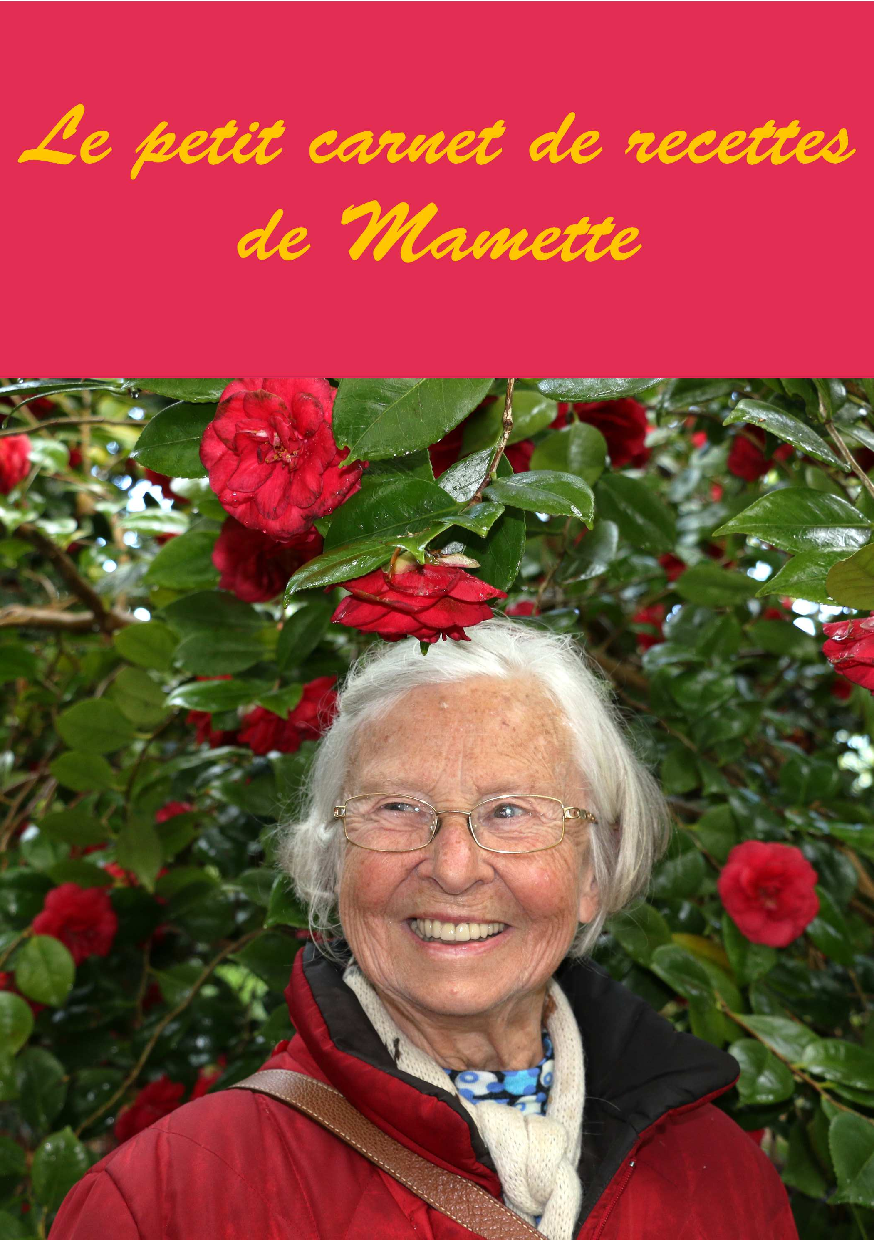
\includepdf{images/couverture2.pdf}
\end{titlepage}

\begin{titlepage}
\parindent=0pt
 \hspace*{\stretch{1}}  %
 \hspace*{\stretch{1}} 
\vspace*{\stretch{1}}

\begin{center}\bfseries\Huge
    Le petit carnet de recettes\\de Mamette
\end{center}
\hrulefill
\vspace*{1cm}
\begin{center}\bfseries\Large
Noël 2015
\end{center}
    
\begin{center}\bfseries\Large
Alice \textsc{Picard}\\
Hanna \textsc{Picard}\\
Mila \textsc{Picard}\\
Nissim \textsc{Picard}\\
Simon \textsc{Picard}
\end{center}
    \vspace*{\stretch{2}}
\begin{flushright}
       
\end{flushright}   
\end{titlepage}
\cleardoublepage

\vspace*{\fill}
\begin{center}
Les prémices de cette retranscription sont nées au Japon lors ce que Alice et Simon étaient dans le monorail de Tokyo, survolant Odaiba. Ce projet est né de l'envie commune de pouvoir profiter des trésors culinaires figurant dans le carnet de leur grand-mère, même s'il est évident qu'ils ne pourront qu'approcher le savoir-faire de Mamette.\\
Ces deux derniers ont rapidement contacté leurs cousins pour mener à bien ce plan, ceux-ci ayant accepté avec enthousiasme.\\


C'est donc avec plaisir et dans une complicité familiale que nous vous proposons de découvrir ce qui se cache effectivement dans ce fameux carnet, en espérant que, comme nous, vous pourrez profiter de cette cuisine légendaire.
\end{center}
\vspace*{\fill}
\cleardoublepage


\tableofcontents
\clearpage

\mainmatter% corps du document
\pagestyle{headings}

\chapter{Entrées}
\begin{figure}[h]
\centering
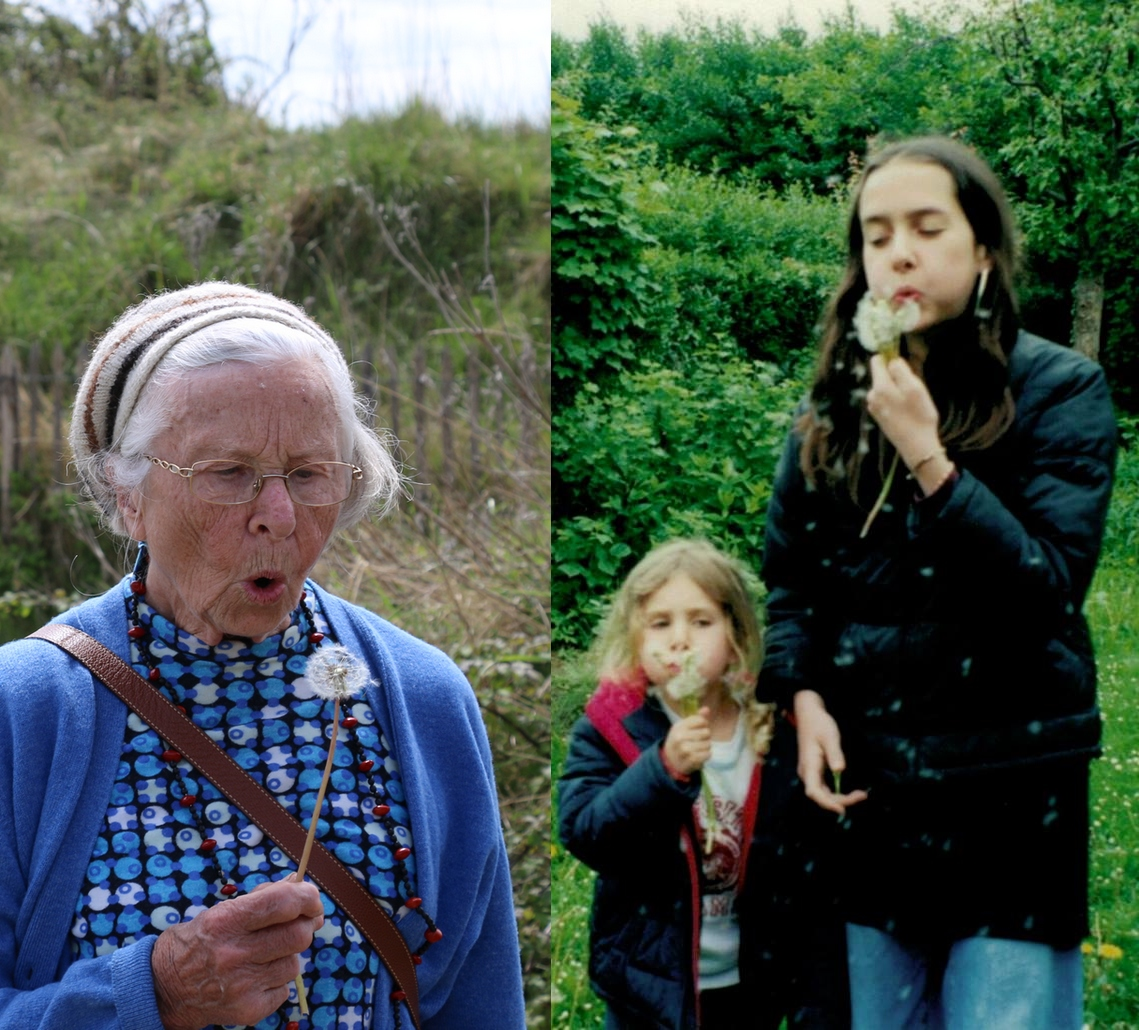
\includegraphics[width=\textwidth]{images/chapter1.jpg}
\end{figure}
\begin{minipage}[c]{\textwidth}
\recette{Potage au curry}
Couper en petits dés : 4 carottes, 2 blancs de poireaux. Emincer un oignon et une gousse d’ail. Cuire $\nicefrac{1}{2}$ heure à petit feu dans un fond d’eau avec 2 cubes de bouillon. Ajouter une cuillère à dessert de curry. \\
Passer au mixage de la soupe. \\
\\

\end{minipage}

\begin{minipage}[c]{\textwidth}
\recette{Mousse de saumon}
\ingredients{
\item Une boite de saumon au naturel 425-450 gr
\item Un sachet de gelée royale
\item Une petite boite de crème épaisse
\item Citron
\item Poivre
}
Diluer la gelée dans $\nicefrac{1}{2}$ L d’eau. Porter à ébullition puis retirer du feu. \\
Ajouter la crème, le saumon égoutté, $\nicefrac{1}{2}$ jus de citron et le poivre. Bien mixer le tout. \\
Mettre au frigo au moins 5h. \\
\\

\end{minipage}

\begin{minipage}[c]{\textwidth}
\recette{Mousse aux foies de volaille}
\ingredients{
\item +- 450 gr de foie
\item 1 sachet de gelée royale
\item 1 petite boite de crème épaisse
\item cognac ou porto
}
Rôtir le foie jusqu’à ce qu’il soit bien cuit. \\
Flamber au cognac ou mettre du porto, ajouter du sel et du poivre. \\
Continuer comme la recette précédente, sans le citron bien sûr. \\
\\

\end{minipage}

\begin{minipage}[c]{\textwidth}
\recette{Salade italienne (excellent !) }
\otor{Bonne Maman Picard}
Couper en petits morceaux : \\
6 grosses pommes de terre cuites\\
La même quantité de betteraves rouges cuites (ou un pot de betteraves au vinaigre)\\
1 dés de céleri rave cuit\\
1 oignon\\
1 pomme crue\\
$\nicefrac{1}{2}$ concombre\\
1 à 2 cuillères à soupe de petits pois (boite)\\
1 boite d’anchois à l’huile\\
Mélanger avec poivre et sel\\
1 à 2 cuillères à soupe de viande cuite\\
Mélanger avec mayonnaise épaisse\\
Décorer avec œuf dur haché, persil, betterave rouge hachée\\
\\

\end{minipage}

\begin{minipage}[c]{\textwidth}
\recette{Soupe à l'orge}
Cuire pendant +- 1 heure de l'orge dans de l'eau avec une gousse d'ail entière, du thym et du laurier. Ne pas saler.\\
Cuire 20 minutes dans de l'eau quelques pommes de terre et un cèleri coupé en morceaux. Saler.\\
Mélanger les deux.\\
\\

\end{minipage}

\begin{minipage}[c]{\textwidth}
\recette{Consommé fin }
\otor{Tilou}
Après les 2h30 de cuisson, ajouter 1 livre ? de bœuf haché et laisser le tout encore cuire 1h.\\
Enlever la viande avant de servir et l’utiliser comme les restes de viande.\\
\\

\end{minipage}

\begin{minipage}[c]{\textwidth}
\recette{Soupe à l’oignon (gruau) }
\otor{Tilou}
Faire revenir un gros oignon dans du beurre (non-bruni !). Le laisser suer à feu très doux. Couvrir d’eau. Ajouter un céleri, une poignée de gruau, du poivre et du sel.\\
Laisser le tout cuire environ 25 minutes. \\
Passer le potage avant de servir.\\
\\

\end{minipage}

\begin{minipage}[c]{\textwidth}
\recette{Soupe au cresson }
\otor{Tilou}
Jeter dans l’eau une botte de cresson, un céleri coupé, du poivre, du sel, du thym, du laurier et une gousse d’ail.\\
Ajouter une poignée de riz quand ça bout.\\
Après environ 25 minutes de cuisson, passer le tout.\\
Au moment de servir, ajouter du liebig et éventuellement un jaune d’œuf dans le fond de la soupière.\\
\\

\end{minipage}

\begin{minipage}[c]{\textwidth}
\recette{Fondues au fromage}
Même pâte que pour les croquettes aux crevettes mais sans les crevettes et en doublant la quantité de fromage (100 gr de gruyère râpé et 50 gr de parmesan râpé). \\
\\
NB : Toujours mettre à demi moins de parmesan par rapport aux autres fromages.\\
\\

\end{minipage}

\begin{minipage}[c]{\textwidth}
\recette{Bouillon }
\otor{Tilou}
Dans l’eau chaude mettre 2-3 carotte, 2-3 poireaux et 1 céleri (environ le tout par parts égales). \\
1,5 livre ? de bouillis au moins.\\
1 livre ? d’os à moelle si possible.\\
Du poivre, du sel, du thym, du laurier et de l’ail.\\
Faire brunir 1 oignon au four jusqu’à ce qu’il soit bien brun.\\
2h30 de cuisson douce.\\
Porter le tout à ébullition puis sur flamme frisonnante.\\
Ajouter des pâtes au moment de servir.\\
\\

\end{minipage}

\begin{minipage}[c]{\textwidth}
\recette{Croquettes aux crevettes}
100 gr de crevettes épluchées (ce qui correspond environ à 250 gr de crevettes non épluchées).  \\
Les faire suer dans un poêlon couvert à feu très doux. \\
Dans un autre poêlon, faire fondre 100 gr de beurre. Y ajouter 100 gr de farine et les trois quarts d’une pinte de lait chaud, du sel, du poivre et 50 gr de fromage. Bien mélanger le tout jusqu’à ce que la pâte se détache de la casserole (sinon elle casse dans la friture). \\
Hors du feu, incorporer un à un, 2 ou 3 jaunes d’œufs à la pâte puis les crevettes.  \\
Remettre un instant sur le feu. \\
Mettre la pâte sur une plaque huilée et mouler les croquettes à l’épaisseur voulue. \\
Laisser refroidir.\\
Passer les croquettes dans la farine, le blanc d’œuf et la chapelure.\\
Laisser reposer.\\
Cuire à la friture.\\
\\

\end{minipage}

\begin{minipage}[c]{\textwidth}
\recette{Bouchées aux crevettes}
Remplir les ridés de la même pâte que pour les croquettes aux crevettes et passer les au four 5 minutes. \\
\\

\end{minipage}

\begin{minipage}[c]{\textwidth}
\recette{Riz de veau aux champignons}
Etape 1: La viande\\
Mettre dégorger la viande dans de l’eau salée ($\nicefrac{1}{2}$ cuillère à soupe de sel).\\
Changer d’eau. \\
Mettre la viande à cuire avec un oignon, une feuille de thym et de laurier, 2 pincées de sel et de poivre.\\
Cuisson une grosse demi-heure.\\
Décortiquer la viande une fois cuite. \\
\\
Etape 2: La sauce (200 gr. de sauce aux champignons pour 350 gr. de riz de veau)\\
Bien laver les champignons à plusieurs eaux.\\
Couper les pieds des têtes, puis égoutter. Faire fondre un gros morceau de beurre jusqu’à ce que ça devienne mousseux. \\
Y faire sauter les champignons à vive allure jusqu’à absorption de tout le beurre. \\
Ajouter 2 cuillères à soupe de farine et $\nicefrac{1}{2}$ jus de citron. Les incorporer totalement. \\
Bien couvrir de lait. Cuire à vive allure 5 minutes en secouant la casserole de temps en temps puis cuire à feu doux 20 à 30 minutes.\\
\\
Etape 3: Les boulettes\\
Pour allonger on peut mettre des boulettes de veau.\\
Mélanger 100 gr de viande de veau haché, 1 jaune d’œuf, du sel et du poivre. \\
Ajouter une poignée de persil haché. Faire absorber du lait par une tranche de mie de pain     au feu avant de l'incorporer à la viande. \\
Former des petites boulettes de viande.\\
Les cuire 5 minutes dans du bouillon (ou un cube dans de l’eau bouillante).\\
\\
Ajouter le riz de veau en tranches et les boulettes à la sauce aux champis ! Bon appétit \\
\\

\end{minipage}

\begin{minipage}[c]{\textwidth}
\recette{Champignons à la grecque}
Dans une casserole versez :\\
un verre d'eau et demie, un demie verre d'huile, un jus de citron, une gousse d'ail brouillé, 6 grains de poivre, 6 grains de cerfeuil, un brins de fenouil, du thym et du laurier. Mélanger et y faire bouillir des petits champignons ou des champignons coupés.\\
Laisser cuire 8 min.\\
Servir bien frais.\\
\\

\end{minipage}

\begin{minipage}[c]{\textwidth}
\recette{Soupe à l'orge}
Faire cuire de l'orge dans de l'eau avec une gouse d'ail entière, du thym et du laurier. Ne pas saler. Faire cuire pendant 1h environ. Faire cuire 20 min dans de l'eau quelques pommes de terre et un cèleri coupé en morceaux, saler et ensuite les rajouter à la soupe.\\
\\

\end{minipage}

\begin{minipage}[c]{\textwidth}
\recette{Potage au pourpier}
Cuir du riz dans du bouillon, avec un cèleri coupé en morceaux. Passez et assaisonnez.\\
Y ajouter le pourpier avant de servir.\\
\\

\end{minipage}

\begin{minipage}[c]{\textwidth}
\recette{Pourpier en légume}
Nettoyer le pourpier divisé en feuilles, le cuire dans du beurre mousseux ,environ 1 litre pour deux personnes.\\
Cuir environ 10 minutes.\\
\\

\end{minipage}

\begin{minipage}[c]{\textwidth}
\recette{Concombre à la grec}
Hors d'œuvre à servir glacé.\\
Détaillez en quartiers deux concombres blancs. Mettre dans une cuisson bouillante de 4dc d'eau, 1dcl d'huile et deux jus de citron, un bouquet garni composé de cèleri, de fenouil, de persil, de thym et de laurier.\\
Ajouter 20 graines de cerfeuil, du poivre et du sel.\\
Cuire à vive allure 10 à 12 minutes.\\
Retirez le bouquet et laissez bien refroidir.\\
\\

\end{minipage}

\begin{minipage}[c]{\textwidth}
\recette{Prunes au vinaigre}
Piquer 4kg de prunes et les équeuter. Ajouter deux litres de vinaigre de vin, 1 kg de sucre Candy blanc, du poivre, deux clous de girofle, du thym et du macis (écorce de muscadier).\\
Le sirop doit bouillir 4 minutes. Ajouter les fruits et faire bouillir. Débarrasser dans une urne.\\
Deux jour après, rangez les prunes en bocaux. Refaire bouillir le jus que vous versez sur les prunes. Bien boucher solidement le lendemain\\
\\

\end{minipage}

\begin{minipage}[c]{\textwidth}
\recette{Morilles}
Les laver à plusieurs reprises à l’eau avec grand soin. Bien éponger. Les sauter au beurre. Comme elles donnent beaucoup d'eau, les faire sauter deux fois puis les égoutter jusqu'à ce qu'elles nagent.\\
Les jeter dans un nouveau beurre brulant pour finir la cuisson.\\
(l'eau sert pour un potage ou une sauce)\\
\\

\end{minipage}

\begin{minipage}[c]{\textwidth}
\recette{Potage de tomate passée}
Ajouter 2 lanières de poivron finement coupé et un peu de riz.\\
Jeter le tout dans la soupe\\
\\

\end{minipage}

\begin{minipage}[c]{\textwidth}
\recette{Cèpes à la bordelaise}
Faire sauter dans de l'huile d'olive bien chaude les têtes de cèpes pendant 10 minutes.\\
Quand elles sont dorées, ajouter de l'ail, du persil, les queues hachées, du sel, du poivre et un jus de citron. Servir bien chaud\\
\\

\end{minipage}

\begin{minipage}[c]{\textwidth}
\recette{Potage tortue}
Faire colorer dans une cuillère a soupe : du beurre, 1 kg d'os concassé, une carotte coupée en petits morceaux, 1 oignon, 1 poireau, 1 petit cèleri et 1 gousse d'ail.\\
Puis versé 2 L d'eau, du thym, du laurier, sel, poivre.\\
Faire cuire à cuisson lente pendant 2h puis ajouter 1 dcl de purée de tomate. Cuire encore 15 min. Passer finement. Couper en dés 100g de tête de veau cuite avec 1 dcl de madere et deux jaunes d'oeufs durs. Couper en quartiers puis chauffer.\\
Lier le potage avec une cuillère a soupe et demie de fécule, délayer dans du madere.\\
Rebouillir 5 min.\\
\\

\end{minipage}

\begin{minipage}[c]{\textwidth}
\recette{Vrai consommé}
Dans un bouillon (cuit 2h30) ajouter une tranche de culotte de bœuf haché de 500g trituré avec deux blancs d'œufs, 1 blanc de poireau haché, une carotte et remettre à cuire pendant 1h30, pas plus !\\
\\

\end{minipage}

\begin{minipage}[c]{\textwidth}
\recette{Potage au champignons}
Dans le bouillon d'oignon verser les champignons hachés et cuits à l'eau légèrement salée avec leur eau de cuisson ou tout simplement l'eau de cuisson seule et employer les champignon pour autre chose, lié avec de la farine.\\
\\

\end{minipage}

\begin{minipage}[c]{\textwidth}
\recette{Cassolettes de saint Flour }
Hacher grossièrement 125g de fromage cantal. Y mélanger dans une terrine bien énergiquement : 250g de fromage blanc égoutté, 2 jaunes d'oeufs et un blanc,1/2 cuillère à café de sel fin,6 à 7 tours de moulin à poivre,1 cuillère à café de ciboulettes haché.\\
Distribuer le tout dans des ramequins. Cuire à feu vif pendant 20 min. Servir en saupoudrant de deux cuillères à café de ciboulette hachées.\\
NB : peut se faire avec du gruyère, du reblochon ou autre fromage cuit\\
\\

\end{minipage}

\begin{minipage}[c]{\textwidth}
\recette{Potage aux lentilles}
Avec des os de mouton, faite un bouillon avec un oignons, deux blancs de poireaux, du thym et du laurier. Cuire 9 pommes de terres. Cuire 250g de lentilles à l'eau froide.\\
Ajouter le tout au reste pour cuire ensemble.\\
\\

\end{minipage}

\begin{minipage}[c]{\textwidth}
\recette{Potage au gruau}
Faire revenir quelques minutes un petit oignon dans une noix de beurre mousseuse.\\
Couvrir d'eau. Jeter y un cèleri finement coupé et une forte pognée de gruaux, du thym, du laurier de l’ail et un cube.\\
Passer et servez\\
\\

\end{minipage}

\begin{minipage}[c]{\textwidth}
\recette{Potage à l'oignion}
Faire revenir dans du beurre mousseau deux oignons hachés jusqu'a ce qu'ils donnent leur suc. Mouiller d'eau bouillante. Laisser cuire 2 minutes. Egoutter. Lier le jus avec 3 cuillères de farine bien délayée et un morceau de liebig.\\
Faire un bon bouillon et servez avec du fromage râpé.\\
\\

\end{minipage}

\begin{minipage}[c]{\textwidth}
\recette{Potage longchamp}
250g de pois réduis en purée\\
100g d’oseilles ? cuites à part au beurre bien fondu. Passer l'oseille et les pois.\\
D’autre part dans deux cubes Liebig, faire cuire du vermissels.\\
Ajouter au potage passé, une noix de beurre et une cuillère de cerfeuil haché, de la\\
crème ou du lait facultatif.\\
\\

\end{minipage}

\begin{minipage}[c]{\textwidth}
\recette{Coulis niçois}
Faire revenir 100g d'oignon dans du beurre mousseux, saupoudrer d’une cuillère de farine. Ensuite, ajouter une boite de purée de tomates ou 5 tomates fraiches et une tranche d'estragon.\\
Verser par dessus 1/2 litre de bouillon ou cube.\\
Finir par un morceau de beurre et servir.\\
\\

\end{minipage}

\begin{minipage}[c]{\textwidth}
\recette{Potage Longchamp}
\ingredients{
\item 250g de pois réduis en purée
\item 100g d’oseille cuite à part au beurre bien fondu
}
Passer l'oseille et les pois\\
D’autre part dans deux cube Liebig faite cuire des vermicelles\\
Ajouter au potage passé + une noix de beurre et une cuillère de cerfeuil haché\\
Crème ou lait facultatif\\
\\

\end{minipage}

\begin{minipage}[c]{\textwidth}
\recette{Potage aux champignons}
Dans le bouillon d'oignions verser les champignons haché est cuit à l'eau légèrement salé\\
Avec leur eau de cuisson ou tout simplement l'eau de cuisson seul et employer les champignons pour autre chose, lié avec de la farine\\
\\

\end{minipage}

\begin{minipage}[c]{\textwidth}
\recette{Potage à l'oignions}
Faire revenir dans du beurre mousseau deux oignions hachée jusqu'à ce qu'ils donnent leur suc\\
Mouiller d'eau bouillante\\
Laisser cuire 2 minutes\\
Égoutter\\
Lier le jus avec 3 cuillères de farine bien délayé\\
Un morceau de Liebig\\
Faite un bon bouillon et servez avec du fromage râpé\\
\\

\end{minipage}

\begin{minipage}[c]{\textwidth}
\recette{Coulis niçois}
Fais revenir 100g d'oignions dans du beurre mousseux\\
Saupoudrez une cuillère de farine\\
Ensuite mettez une boite de purée de tomate ou 5 tomates fraîches et une tranche d'estragon\\
Verser par dessus 1/2 litre de bouillon ou cube\\
Finir par un morceau de beurre et servir\\
\\

\end{minipage}

\begin{minipage}[c]{\textwidth}
\recette{Œufs Mirabeau}
Longuement battre 4 œufs avec un demi verre de lait tiède\\
150g de fromage râpé\\
Une cuillère de beurre fondu et du poivre\\
Mettre dans des ramequins beurrés\\
Cuire au bain mari dans 2 cm d'eau au four 15 à 20 minutes\\
démouler, servir avec de la béchamel ou de la sauce tomate\\
\\

\end{minipage}

\begin{minipage}[c]{\textwidth}
\recette{Œufs mollet cressonnières}
Cuire les œufs 5 min et les rafraichir avant de les pelés\\
Nettoyer une botte de cressons\\
La jeter dans de l'eau bouillante salée\\
Égoutter de suite et rafraichir\\
Exprimé? L’eau \\
Passer au tournis et mélanger à une sauce mayonnaise très relevé\\
\\

\end{minipage}

\begin{minipage}[c]{\textwidth}
\recette{Guacamole (entré mexicaine)}
Ecraser 3 avocats mur\\
Mélanger avec 25g d'oignons rouge hachée,\\
Quelques gouttes de tabasco,\\
Le jus d’ un demie citron\\
1/2 de cuillère à café d'ail en poudre,\\
1/2 cuillère à café de curry en poudre\\
Une pincée de sel\\
\\

\end{minipage}

\begin{minipage}[c]{\textwidth}
\recette{Confiture d'oignions}
Émincé 2 gros oignions ou plus\\
Les faire revenir dans une noix de beurre en les saupoudrant de 2 cuillère à soupe de sucre\\
Laisser cuire 10 min\\
Les mouiller avec 4 cuillère à soupe de vinaigre de vin, un demie litre de vin rouge, 4 cuillère à soupe de grenadine ou 4 cuillère à café de gelé de groseille.\\
Saupoudrez de thym laurier sel poivre\\
Laisser réduire 1/2 h jusqu'à obtenir une masse rouge\\
\\

\end{minipage}

\begin{minipage}[c]{\textwidth}
\recette{Beignet soufflé au parmesan}
Mettre dans une casserole 60g de beurre, du sel, du poivre, de la muscat, du paprika et les 3/4 d'un verre contenant un mélange lait et eau\\
Faire bouillir\\
Ajouter en remuant a la spatule 150g de farine jusqu’à obtenir une pâte épaisse\\
Continuer à battre jusqu’à ce que la pâte épaisse se détache en boule de la casserole\\
Hors du feu ajouter deux œufs à la fois en remuant jusqu'à   ce qu'elle redevienne épaisse. Ajouter en battant 60g de parmesan râpé\\
Cuire à la friture des boulettes de pate grosse comme une noix\\
Servez bien chaud sur serviette pliée ou papier absorbant\\
\\

\end{minipage}

\begin{minipage}[c]{\textwidth}
\recette{Conserve de cornichons et petits oignons}
Les petits oignons doivent être pelés. Les mettre dans une terrine avec une poignée de sel - bien mélanger - laisser reposer une nuit. \\
Le lendemain, bien essuyer 1 ou deux fois selon la saleté. Les mettre en bocal. Ajouter du vinaigre, de l'estragon, du fenouil  éventuellement un piment.\\
\\

\end{minipage}

\begin{minipage}[c]{\textwidth}
\recette{Brochette créole }
\ingredients[(4 personnes)]{
\item 16 petits cubes de gouda d’environ 1 cm 50
\item 16 très fine tranches de lard fumé
\item 4 tranches d'ananas et 4 piques à brochette
}
Enroulez les cubes de fromage entièrement dans le lard\\
Coupé les tranche d'ananas En cube,\\
Enfilé alternativement les cube de fromage enroulé de lard et ceux d'ananas\\
Mettre 10 minutes au grill ou sur un poêle chaude\\
Retourner à mi-cuisson\\
Servir très chaud (avec du riz ça peut faire un repas complet)\\
\\

\end{minipage}



\chapter{Plats}
\begin{figure}[h]
\centering
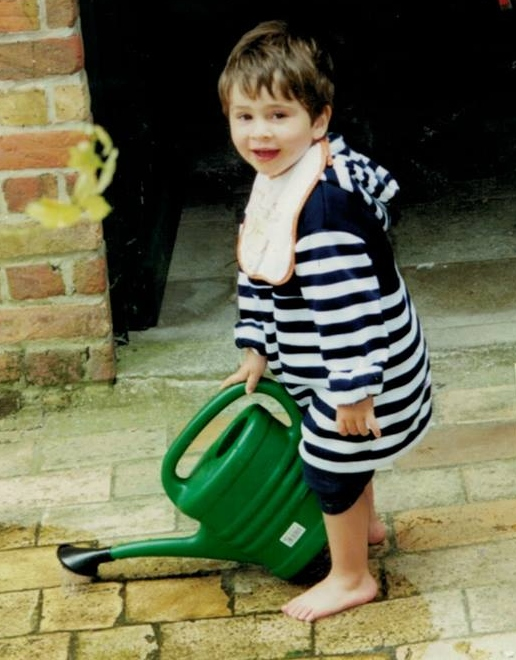
\includegraphics[width=0.85\textwidth]{images/chapter2.jpg}
\end{figure}
\begin{minipage}[c]{\textwidth}
\recette{Moules}
Laver et gratter les moules.\\
Les plonger dans de l’eau salée. Egoutter \\
Faire revenir un oignon coupé dans du beurre. \\
$\nicefrac{1}{2}$ céleri + persil. Faire revenir dans le beurre sans roussir. \\
Mijoter les moules. \\
Cuisson : environ 10 minutes\\
\\

\end{minipage}

\begin{minipage}[c]{\textwidth}
\recette{Soufflé au homard }
\ingredients[(6 personnes)]{
\item Bisque de homard : $\nicefrac{1}{2}$ à $\nicefrac{3}{4}$ de boite
\item 4 pommes
\item Gruyère râpé : 80 gr
\item 4 blancs d’œufs
\item Beurre
}
Verser $\nicefrac{1}{2}$ à $\nicefrac{3}{4}$ d’une boite de bisque de homard sans diluer dans une casserole de 1L, avec $\nicefrac{1}{4}$ de verre d’eau chaude. Chauffer à feu doux en mélangeant à la spatule. \\
Ecarter du feu. Ajouter les 4 pommes en mélangeant vite, puis ajouter le gruyère râpé et du poivre et du sel. \\
Battre très fermes 4 blancs d’œufs. Mélanger 2 cuillères à soupe de blanc battu à la préparation avec la cuillère puis le reste délicatement à la fourchette. \\
Beurrer le moule. Y verser le mélange aux $\nicefrac{3}{4}$ de la hauteur. \\
Cuire à feu moyen 15 à 20 min. \\
\\

\end{minipage}

\begin{minipage}[c]{\textwidth}
\recette{Foie}
Passer les tranches de foie dans de la farine avant de les faire cuire à la poêle. \\
\\

\end{minipage}

\begin{minipage}[c]{\textwidth}
\recette{Cassolette au homard}
Verser 1 boite de bisque de homard « Liebig » dans une casserole. Chauffer doucement en mélangeant. \\
Prélever quelques cuillérées de bisque éclaircies à l’eau chaude (un peu).\\
Ajouter 2 œufs frais et mélanger doucement au fouet sans faire mousser. \\
Incorporer le reste de la bisque. \\
Verser dans des ramequins remplis aux $\nicefrac{3}{4}$. Les poser dans un plat au four avec de l’eau chaude jusqu’à mi hauteur des ramequins. Cuire à four chaud pendant 25 minutes. \\
\\

\end{minipage}

\begin{minipage}[c]{\textwidth}
\recette{Spaghettis à l’italienne}
\ingredients{
\item Spaghettis
\item Lait
\item Levure
\item 2 œufs
\item Echalote
\item Jambon ou langue 
\item Sauce tomate
}
Cuire les spaghettis dans du lait (1/2 litre pour une poignée).\\
Ajouter hors du feu une cuillère de levure, 2 œufs battus et l’échalote hachée.\\
Hacher finement du jambon ou de la langue. Mélanger.\\
Cuire une heure au bain marie dans un moule à cheminée beurré. \\
Arroser de sauce tomate après cuisson. \\
\\

\end{minipage}

\begin{minipage}[c]{\textwidth}
\recette{Les œufs à la milanaise}
Beurrer le fond d’un plat à gratin. Y disposer de fines tranches de pain. \\
Recouvrir d’une couche de fines lamelles de gruyères, d’une couche de langue fumée hachée, d’une couche de sauce tomate. Casser dessus (sans crever le jaune) 3 ou 4 œufs. \\
Assaisonner. \\
Cuire à four doux pendant 10 minutes\\
\\

\end{minipage}

\begin{minipage}[c]{\textwidth}
\recette{Pontis auvergnat}
Dans un peu de beurre, faire remuer 3 rog lard fumé coupé en dés. \\
Ajouter un oignon moyen et une poignée de fines herbes hachées.\\
Cuire en mijotant avec un peu d’eau, du poivre et du sel. \\
Délayer deux tasses à thé de farine dans un bol de lait, ajouter 2 ou 3 jaunes d’œufs et les blancs battus en neige.\\
Mélanger le tout, puis mettre à cuire $\nicefrac{3}{4}$ d’heure dans un moule à soufflé grassement beurré. \\
\\

\end{minipage}

\begin{minipage}[c]{\textwidth}
\recette{Gratin dauphinois}
\ingredients{
\item 1 kg de pommes de terre
\item 2 œufs
\item 125 g de gruyère râpé
\item 75g de beurre
\item $\nicefrac{1}{2}$ litre de lait
\item Sel, poivre, muscade
}
Eplucher les pommes de terre et les couper en rondelles fines.\\
Battre les œufs en omelette et y mélanger le lait, sel, poivre et muscade. \\
Beurrer un plat allant au four, y placer une couche de pomme de terre. Arroser avec le mélange lait/œufs puis saupoudrer de râpé. Recommencer jusqu’à remplir le plat. \\
Arroser de beurre fondu sur le dessus du plat recouvert du reste de râpé. \\
Cuire à four chaud 60 à 80 min.\\
A manger comme entrée ou avec un plat de viande.\\
\\

\end{minipage}

\begin{minipage}[c]{\textwidth}
\recette{Petits pois à la française}
Faire revenir 4 tout petits oignons dans du beurre.\\
Ajouter quelques feuilles de laitue dans le fond et un peu d’eau si nécessaire.\\
1 bouquet de persil lié.\\
Verser les pois et 2 sucres. Laisser cuire à feu très doux une petite heure.\\
Retirer la laitue avant de servir.\\
\\

\end{minipage}

\begin{minipage}[c]{\textwidth}
\recette{Pate à frire très légère}
\ingredients{
\item 125 g de farine
\item 2/3 de verre d’eau, bière ou vin blanc
\item 1 cuillère d’huile ou de beurre fondu
\item 2 blancs d’œufs
}
Délayer la farine avec le liquide choisit plus une pincée de sel. Ajouter du beurre ou de l’huile quand c’est bien délayé.\\
Reposer une heure. \\
Au moment d’utiliser la pâte, y ajouter les deux blancs. Battre en neige ferme. \\
\\

\end{minipage}

\begin{minipage}[c]{\textwidth}
\recette{Beignets de quenelles de volailles}
\ingredients{
\item 1/2 boite de quenelles de +/- 35 g chacune
\item Pâte à frire très légère (recette précédente)
}
Égoutter les quenelles, puis les faire macérer une heure dans un peu de madère. Egoutter à nouveau. \\
Frire à l’huile après les avoir plongé une à une dans la pâte à beignet. \\
Egoutter et décorer de persil frit.\\
\\

\end{minipage}

\begin{minipage}[c]{\textwidth}
\recette{Cuisson du chou fleur}
Le mettre dan l'eau froide, portez à ébullition. Quand elle bout, jetez cette eau et la remplacer par de l'eau chaude.\\
(Ceci supprime la mauvaise odeur, idem pour les choux de Bruxelles)\\
\\

\end{minipage}

\begin{minipage}[c]{\textwidth}
\recette{Médaillon de veau}
Médaillons d’environ 4 cm d’épaisseur cerclés d’une bande de lard. \\
Faire fondre dans une cocotte un bon morceau de beurre, y mettre les médaillons et cuire environ 30 min (cocotte fermé) après les avoir doré des deux cotés.\\
Laver 250 g de champignons et jeter dans l’eau bouillante légèrement vinaigrée.  Faire bouillir 5 minutes, puis les égoutter dans un torchon. \\
Mettre les champignons dans la cocotte à coté des médaillons 5 minutes.\\
Retirer le tout, mettre dans la cocotte un bol de crème sur feu très doux sans faire bouillir mais lentement chauffé. \\
Y ajouter la viande et les champignons et servir.\\
\\

\end{minipage}

\begin{minipage}[c]{\textwidth}
\recette{Soufflé de jambon}
\ingredients{
\item 2 œufs 
\item 2 cuillères à soupe de farine
\item $\nicefrac{1}{2}$ L de lait
\item 2 cuillères de porto blanc ou Vermouth blanc
\item Beurre
\item Jambon en dés (250 gr)
\item Gruyère râpé
\item Sauce Mormay
}
Pâte : délayer deux jaunes d’œufs dans deux cuillères à soupe de farine tamisée avec \\
$\nicefrac{1}{2}$ L de lait bouilli et refroidi. Ajouter en battant 2 cuillères de porto blanc ou de vermouth blanc, du sel et du poivre puis les 2 blancs battus en neige ferme.\\
Beurrer un moule. Au fond, y placer une fine couche de jambon coupé en petits dés. Saupoudrer de gruyère râpé, puis verser une couche de pâte. Continuer en alternant les trois couches et terminer par la pâte.\\
Cuire au bain marie environ 1 heure. \\
Démouler sur un plat chaud et napper d’une sauce Mormay (pour sa confection, voir recette de la tarte aux asperges-Béchamel au lait et fromage râpe)\\
\\

\end{minipage}

\begin{minipage}[c]{\textwidth}
\recette{Timbale au jambon}
Cuire à l’eau salée 250g de coquillettes. Les égoutter dès qu’elles sont souples sous le doigt.\\
Rincer à l’eau froide et de nouveau égoutter. \\
Hacher assez gros 250 g de jambon maigre. Mélanger aux coquillettes avec 2 œufs battus et 125g de Gruyère râpé. \\
Beurrer largement le moule à cheminée ou à charlotte, et y verser la préparation. \\
Cuire au four ou au bain marie 30 minutes, puis laisser reposer dans le moule au bain marie. Après 10 minutes, démouler sur un plat préchauffé. \\
Verser dessus une sauce Aurore (Béchamel au lait et sauce tomate en quantité égale et chaude.)\\
\\

\end{minipage}

\begin{minipage}[c]{\textwidth}
\recette{Mousse de Jambon Florentine}
\ingredients{
\item Beurre
\item 3 cuillères de farine
\item 1,5 verre de lait
\item 1 cuillère de concentré de tomates
\item 300 gr de jambon maigre
\item 1-2 cuillère de crème épaisse
\item 2 œufs
\item Poivre
\item Epinards au beurre ou à la crème
}
Dans une casserole, ajouter 3 cuillères de beurre et de la farine en même quantité. Délayer à feu doux avec 1,5 verre de lait froid. \\
Laisser épaissir en tournant, puis ajouter une cuillère de concentré de tomates. \\
Cuire à l’étouffé environ 15 minutes avant d’ajouter le jambon maigre haché finement. \\
Ajouter rapidement  de 2 à 4 cuillères de beurre et 1 à 2 cuillères de crème épaisse. Réchauffer puis incorporer hors du feu les deux jaunes puis les deux blancs en neige ferme. Poivrer, puis verser dans un moule droit bien beurré. Cuire 15 min à four assez chaud. Démouler et entourer d’épinards au beurre ou à la crème. \\
On peut cuire la mousse dans une timbale en porcelaine en y ajoutant un blanc d’œuf en neige. Servir alors les épinards à part.\\
\\

\end{minipage}

\begin{minipage}[c]{\textwidth}
\recette{Tarte aux asperges }
\ingredients{
\item Pâte : 
\item 200 gr de farine
\item 150 gr de beurre
\item 1 petit verre d’eau salée.
}
Mélanger rapidement le tout, puis laisser reposer une heure. \\
Etaler dans un moule (29 cm). \\
Piquer, et cuire à four chaud pendant 20 min. \\
Cuire les asperges pelées dans l’eau légèrement salée de 20 à 30 min.\\
Déposer sur la pâte cuite les asperges cuites et coupées. \\
Recouvrir de sauce Mormay (voir ci dessous).\\
Glisser au four chaud quelques minutes pour gratiner (se réchauffe facilement si il en reste).\\
Sauce mormay :\\
Dans 30 gr de beurre fondu, jeter 30 gr de farine et mélanger. \\
Ajouter petit à petit 125 gr de crème ou lait condensé non sucré et 50 gr de fromage râpé. \\
En faire une crème épaisse. \\
\\

\end{minipage}

\begin{minipage}[c]{\textwidth}
\recette{Porc Maréchal}
(convient aussi pour un rôti de veau)\\
Cuire à four chaud un filet de porc de 1 kg ou un rôti un peu allongé, avec une cuillère de beurre pendant une heure (pas plus).\\
Laver 500 gr de champignons et les cuire au beurre puis les hacher avec 250 gr de jambon maigre. \\
Faire une béchamel épaisse : à 2 cuillères de beurre fondu, ajouter 5 cuillères de farine et réchauffer, tout en y versant progressivement $\nicefrac{1}{2}$ litre de lait. \\
Mélanger le haché dans cette sauce. Saler, poivrer et ajouter une pointe de muscade. Découper le rôti cuit en tranches pas trop fines et les recoller en utilisant le hachis entre chaque tranche.\\
Une fois le rôti remodelé, verser sur les cotés le reste du hachis et saupoudrer de 100g de fromage râpé (gruyère ou parmesan). \\
Faire gratiner au four chaud jusqu’à ce que le rôti et le fromage soient bien dorés. \\
\\

\end{minipage}

\begin{minipage}[c]{\textwidth}
\recette{Framboise surprise}
Moudre 125 gr d’amandes ou de noix mélangé à 100 g de sucre fin. Ajouter 3 jaunes d’œufs et bien mélanger. \\
Battre les 3 blancs en neige ferme et les ajouter au mélange très doucement. \\
Verser dans un plat qui va au four dans lequel on a mis 150 gr de framboises. Cuire 10 à 15 minutes à four doux.\\
Se déguste chaud ou froid !\\
\\

\end{minipage}

\begin{minipage}[c]{\textwidth}
\recette{Tajine de poulet au tomate et miel}
\ingredients{
\item 1,5 kg de poulet (cuisses par exemple)
\item 2 boites de tomates pelées
\item 2 oignons émincés
\item 4 cuillères à soupe de pignons
\item 2 cuillères à soupe de miel
\item Huile d’olive
\item Beurre
\item $\nicefrac{1}{2}$ cuillère à café de 4 épices
\item 2 cuillères à soupe de persil plat haché
}
Egoutter les tomates, les couper en deux. \\
Si c’est des grandes cuisses, les couper en deux aux jointures. Les faire dorer des 2 côtés dans l’huile et le beurre chauds. Retirer quand elles sont colorées et jeter l’excès de graisse. Faire revenir 2 oignons hachés saupoudrés de 4 épices.\\
Rajouter le poulet-tomates, le sel et le poivre, faire mijoter 45 minutes à feu doux en retournant les morceaux à mi cuisson.\\
Griller les pignons sans graisse. \\
Retirer le poulet, ajouter le miel et laisser mijoter 2 minutes. \\
Rajouter les morceaux de poulet et les pignons. Saupoudrer le tout de persil plat. \\
NB : c’est très bon et ca se surgèle facilement ! \\
\\

\end{minipage}

\begin{minipage}[c]{\textwidth}
\recette{Osso buco }
1. Mirepoix: \\
2 blancs poiveraux\\
2 carottes \\
2 oignons\\
2 branches de céleri\\
Tous ces ingrédients hachés fins. \\
100 gr de lard fumé haché\\
1 cuillère à soupe d’huile d’olive\\
Laurier et thym\\
Faire cuire à couvert très doucement jusqu’à ce que les légumes soient fondus, garder au chaud. \\
2. Jarret de veau : \\
6 tranches de 3 cuissons différentes. Les fariner, ajouter poivre et sel. Faire dorer à la poêle doucement dans 3 cuillères à soupe d’huile et 3 cuillères à soupe de beurre. \\
3. Ajouter la viande à la Mirepoix et $\nicefrac{1}{2}$ verre de vin blanc sec et faire mijoter jusqu’au moment où le liquide a réduit d’1/4. \\
Y ajouter 2 cuillères à soupe de purée tomate et une tasse de bouillon. \\
4. Faire mijoter 1h15. Passer le jus et faire réduire d’1/4. \\
Parsemer la viande de persil, d’ail et de zestes de citron hachés finement. \\
Napper les morceaux de veau de la sauce et servir bien chaud !\\
\\

\end{minipage}

\begin{minipage}[c]{\textwidth}
\recette{Champignons à la grecque}
\ingredients{
\item 1,5 verre d'eau
\item 1/2 verre d'huile
\item Le jus d’1 citron
\item 1 gousse d'ail brouillé
\item 6 grains de poivre
\item 6 grains de cerfeuil
\item 1 brin de fenouil
\item Du thym et du laurier
}
Versez le tout dans un casserole d'eau.\\
Mélanger et y faire bouillir les champignons petits ou coupés.\\
Cuire 8 minutes puis servir bien frais.\\
\\

\end{minipage}

\begin{minipage}[c]{\textwidth}
\recette{Tarte à la moelle}
1. Pâte : brisée. \\
250 gr (2x $\nicefrac{1}{2}$ tasse à thé) de farine\\
1 cuillère à café de sel\\
125 gr de beurre\\
Rouler le mélange avec les doigts jusqu’à obtenir une semoule. \\
Verser +- 1 verre d’eau mélangé pour avoir une pâte légère qu’on peut rouler facilement. Pétrir légèrement et reposer. \\
Beurrer le moule à tarte et fariner (+- 20 cm de diamètre et 2,5 cm de haut). Piquer, et bien appliquer sur les bords. \\
2. Garniture :\\
- tremper dans l’eau 50 gr de baguette ou petits pains (sandwich). \\
- macérer dans du vin rouge ordinaire +- 125 gr de raisin Corinthe toute une nuit\\
- oignons : 1 kg épluché et haché doré dans 3 cuillères à soupe d’huile. Ajouter 2 cuillères à   soupe de sucre\\
- moelle : évider 2 à 3 os pour obtenir +- 100-150 gr de moelle. Faire fondre à feu doux quelques minutes. \\
- exprimer l’eau du pain\\
- Ajouter les raisins égouttés\\
- Ajouter aux oignons\\
- Ajouter la moelle\\
Mélanger le tout à feu doux et mouler la pâte dans un moule enfariné de 26 cm +-. Piquer le fond et y verser le mélange. En garder un peu pour faire grésiller sur la tarte garnie. \\
Cuire à feu chaud 25 à 30 minutes. \\
\\

\end{minipage}

\begin{minipage}[c]{\textwidth}
\recette{Gâteau de crêpes}
Empiler en alternance 1 crêpe, 1 tranche de jambon, 1 crêpe, 1 tranche de jambon, etc. Jusqu’à ce que ça forme un gâteau. \\
Couler dessus une sauce au fromage faite en mélangeant dans un poêlon 35 gr de beurre, 1 cuillère à soupe de farine, du fromage, 1 jaune d’œuf et 1 bonne tasse de lait.\\
Découper comme un gâteau pour servir.\\
\\

\end{minipage}

\begin{minipage}[c]{\textwidth}
\recette{Poulet en gelée}
Dans une marmite : 200 gr de couenne de lard maigre (Facultatif : $\nicefrac{1}{2}$ pied de veau), 2-3 carottes, 2 oignons, 2 gousses d’ail, thym, laurier, persil, sel, poivre, 2 verres de vin blanc courant mais sec. Y poser le poulet et ajouter assez d’eau pour qu’il baigne.\\
Faire bouillir à petit feu +- 2h15. \\
Sortir le poulet et enlever toute la peau. Le désosser. \\
Remettre le bouillon au feu et laisser réduire pour avoir une gelée bien ferme. Passer dans la passoire fine. \\
Verser sur le poulet désossé et nu dans une terrine, les plus beaux morceaux en dessous. \\
En refroidissant, il y aura de la gelée sur le poulet. \\
Avant de servir, plonger la terrine 1 minute dans de l’eau chaude pour détacher le poulet et le renverser sur le plat de service. Y verser de la gelée (mais pas trop.) \\
Faire refroidir à l’air et servir avec une bonne salade. Mmm !\\
\\

\end{minipage}

\begin{minipage}[c]{\textwidth}
\recette{Courgettes aux tomates}
Faire fondre un peu de beurre dans un poêlon avec un de l’oignon finement haché (en quantité, l’équivalent d’une gousse d’ail). Y mettre les tomates dessus et les courgettes bien lavées et coupées en tranches. Ajouter in peu d’ail bien haché, du sel et du poivre. \\
Faire cuire 30 à 45 minutes.\\
Quand c’est cuit, mettre dans un plat à gratin et couler par dessus 2 œufs entiers battus.\\
Passer au four 5 minutes avant de servir. \\
\\

\end{minipage}

\begin{minipage}[c]{\textwidth}
\recette{Scaroles au fromage}
Cuire les scaroles à l'eau et les placez ensuite dans un pat allant au four.\\
Les recouvrir d'une sauce au fromage : une cuillère à café de farine, du beure, du fromage râpé, un jaune d'œuf.Laissez dorer au four.\\
\\

\end{minipage}

\begin{minipage}[c]{\textwidth}
\recette{Quiche de Lorraine}
Pâte :\\
\\
Faire un puits avec 250 gr de farine, y mettre 130 gr de beurre travaillé à la main, une pincée de sel et un petit verre de lait ou d’eau tiède. Mélanger le tout sans toutefois trop travailler la pâte. \\
La laisser reposer 2h au frais.\\
\\
Crème : \\
\\
Délayer 40 gr de farine avec un peu de crème (ou de lait).\\
Casser les 3 œufs et les travailler 5 minutes avec une cuillère en bois. Y ajouter le reste de crème et une pincée de sel. \\
Couper en petits carrés 100 gr de lard fumé.\\
Chauffer 5 gr de saindoux dans un poêlon. Y faire dorer le lard, l’égoutter et le mélanger avec la crème en remuant bien. \\
Etendre la pâte et la mouler dans une forme à tarte de 30 cm de diamètre préalablement beurrée.\\
Y verser la crème et cuire le tout à four chaud environ 30 minutes.\\
Servir chaud avec des épinards à la crème ou de la purée de pois.\\
\\
NB : Si la quiche se colore trop, la couvrir d’un papier beurré dès qu’elle à fait croûte.\\
\\

\end{minipage}

\begin{minipage}[c]{\textwidth}
\recette{Quenelles Rumsteak Américain }
Hacher un beefsteak d’un livre ?.\\
Y incorporer de la mie de pain rassis, 2 œufs entiers et du persil haché. \\
Bien mélanger.\\
Cuire au grill préalablement chauffé.\\
Sauter au beurre à la poêle. \\
\\

\end{minipage}

\begin{minipage}[c]{\textwidth}
\recette{Steak américain}
125 gr de viande hachée par personne.\\
2 jaunes d’œuf par 250 gr de viande.\\
Sel et poivre.\\
Ajouter une cuillère à café de moutarde délayée, de l’huile cf. mayonnaise (??), du vinaigre aromatisé, 1 filet de sauce anglaise, des petits cornichons hachés ou des câpres.\\
Servir avec des petits oignons sur le plat.\\
\\

\end{minipage}

\begin{minipage}[c]{\textwidth}
\recette{Pommes de terre à la mode de Prague }
Cuire à l’eau pendant 25 minutes des pommes de terre moyennes dans leurs pelures.\\
Cuire 6 œufs durs (10 min. dans l’eau bouillante).\\
Eplucher les pommes de terre et les œufs. \\
Couper les deux en rondelles d’1/2 cm. \\
Disposer une rangée de pomme de terre dans le fond du plat à gratin. Saler et poivrer. \\
Recouvrir d’une couche de crème fraiche, puis des œufs. Saler et poivrer. \\
Recouvrir du reste de pommes de terre. Saler.\\
Recouvrir du reste de crème (il en faut 150 gr pas trop épaisse.) saupoudrer de 50 gr de gruyères ou de parmesan râpé.\\
Mettre 10 minuntes à four chaud pour bien dorer. \\
Servir chaud !\\
\\

\end{minipage}

\begin{minipage}[c]{\textwidth}
\recette{Choufleur en timbale}
Cuire le chou à l'eau et le déposer par lit dans un moule beurré. Alternez avec un lit de viande haché jusqu'a épuisement.\\
Cuir au bain marie pendant 45 minutes. Servir avec une sauce tomate\\
\\

\end{minipage}

\begin{minipage}[c]{\textwidth}
\recette{Soufflé au fromage }
\ingredients[(6 personnes)]{
\item 250 gr de crème
\item 125 gr de gruyère râpé
\item 30 gr de beurre
\item 25 gr de parmesan râpé
\item 25 gr de fécule
\item 6 œufs frais
\item Muscade, sel et poivre. 
}
Mettre dans une casserole la crème, le beurre et la fécule.\\
Chauffer en mélangeant constamment jusqu'a obtenir une pâte lisse, assaisonner.\\
Eloigner la casserole du feu, y  ajouter les jaunes d’œufs et le fromage. Mélanger le tout.\\
Battre les blancs en neige bien ferme, les incorporer légèrement au mélange.\\
Verser le tout dans un plat creux légèrement beurré et mettre au four pas trop chaud pendant 25 à 30 min. \\
\\

\end{minipage}

\begin{minipage}[c]{\textwidth}
\recette{Pomme de terre soufflées}
Couper des pommes de terre en rondelles, les sécher et les étaler. Faire chauffer de l'huile pas trop chaude, y ajouter les rondelles une à une, cuire deux minutes à petit feu, enlever la bassine et laissez cuire 7 minutes.\\
Réchauffer le tout à gaz et ajoutez l'huile continuellement en tenant la bassine par les deux hanses. Lorsque les pommes de terre sont dorées et gonflent, retirer et saler.\\
\\

\end{minipage}

\begin{minipage}[c]{\textwidth}
\recette{Choux frisons}
Détacher les feuilles, blanchir à l'eau bouillante et puis les rafraichir. Hacher grossièrement. Mettre dans une casserole un peu de graisse, une demi verre d'eau et les choux. Assaisonner et ajouter deux ou trois cuillères de riz. Couvrir 20 min. Découvrir et saupoudrer de fromage. Gratiner au four quelques minutes\\
\\

\end{minipage}

\begin{minipage}[c]{\textwidth}
\recette{Semoule}
Faire bouillir un demi litre de lait avec 2 cuillères à soupe de sucre, ajouter 2 et demie cuillères à soupe de semoule en pluie et tournez avec le fouet jusqu'à ce que ca devienne très épais .\\
Goutez pour vérifier si c'est cuit, ajouter une poignée de raisin sec passé à l'eau chaude et un paquet de sucre vanillé. Retirez du feu et ajouter un jaune d'œuf. Incorporez un ou deux blanc battu en neige. Versez dans un plat et garnir de cassonade qui va fondre à la chaleur de la semoule.\\
\\

\end{minipage}

\begin{minipage}[c]{\textwidth}
\recette{Oignions à la monégasque}
Epluchez un litre d'oignions de même grosseur. Les mettre dans une casserole avec 1/3 de litre d'eau, deux verres à  porto de vinaigre blanc, 3 cuillères a soupe d'huile, 50g de sucre en poudre, 3 cuillères à soupe de purée de tomate, 1 petit bouquet de thym, du laurier, du persil, du poivre et du sel et 75 gramme de raisins secs. Faire bouillir et laisser cuir 1h30.\\
Servir froid dans un vasque en crystal\\
\\

\end{minipage}

\begin{minipage}[c]{\textwidth}
\recette{Poivron cru}
Couper en fines lamelles après avoir enlevé les pépins. Faire passer la nuit à la cave avec du sel et de l'huile (couvrir d'huile). Le lendemain ajouter de vinaigre.\\
\\

\end{minipage}

\begin{minipage}[c]{\textwidth}
\recette{Chanterelles}
Bien les laver et les presser dans un linge, les faire blanchir quelques instants à l'eau bouillante et salée. Les sauter au beurre avec du jus de citron à feu doux environ 20 minutes. Se sert mélangé à du jus de rôtis de veau et atour du rôtis avec une omelette ou des oeufs brouillés.\\
\\

\end{minipage}

\begin{minipage}[c]{\textwidth}
\recette{Cèpes farcies}
Bien laver. Séparer les tètes des queues que l'on réserve pour la farce. Hacher finement de l'oseil, du lard, des échalotes, de l'ail, de la ciboulette et du persil. Mélanger avec les queues. barder de lard le fond de la casserole. Disposer une bonne couche de champignons puis une couche de farce , recommencez jusqu'à épuisement.\\
Faire cuire 2-3 heures à petit feu.\\
Ajouter ensuite des pommes de terre bien rondes au dessus puis faire cuire encore deux heures.\\
\\

\end{minipage}

\begin{minipage}[c]{\textwidth}
\recette{Chateaubriand aux champignons}
Enlever les queues, éplucher les tête, couper en morceaux et tremper dans de l'eau acidulée. Mettre dan une petite casserole du jus de viande, un morceaux de beurre, du sel, du poivre et un petit verre de madère. Cuire à feu doux. \\
Préparer le bifsteak : Griller dans une poile noir, puis sauter au beurre. Pendant ce temps, faire cuir les champignons dans la sauce. Dresser le steak sur un plat garnir de champignons. Servir la sauce à part.\\
\\

\end{minipage}

\begin{minipage}[c]{\textwidth}
\recette{L’omelette mousseline}
Battre très ferme les blancs en neige de 6 œufs. Dans un bol battre les jaunes avec 100g de sucre puis incorporer les blancs, verser le tout dans un poêle beurrée.\\
Une fois cuite, passer au four pour dorer le second côté. Porter sur un plat chaud\\
Verser 3 cuillères de confiture en languette et replier vers le milieu les deux bords.\\
Arroser de kirsch enflammé\\
\\

\end{minipage}

\begin{minipage}[c]{\textwidth}
\recette{Aubergines niçoises}
Ouvrir six petites aubergines en deux en longueur, les faire revenir dans une poêle à l'huile pendant 10 min. Videz le milieu qu'il faut réserver pour la farce.\\
Mélangez le milieu avec 125g d’anchois ou de viande hachée, 30g de mie de pain (bouillie dans du lait jusqu'a ce qu'elle devienne une pate), une gousse d’ail finement haché, du sel et du poivre. Dresser les aubergines dans un plat à gratiné à côté de 500g de petites tomates ouvertes et vidées. Remplir les aubergines et les tomates de farce. Remettre le couvercle des aubergines/tomates et beurrer. Porter au four bien chaud qu'on baisse en enfournant. cuisson 1/2 heure. Servir brulant.\\
\\

\end{minipage}

\begin{minipage}[c]{\textwidth}
\recette{Bordure au fromage - ragout de crevettes ou champignons}
\ingredients{
\item 1/4 de litre de lait
\item 40g de beurre
\item 40g de farine
\item 100g de fromage rapé
\item 2 oeuf
\item Poivre et sel
}
Préparation : Faire fondre le beurre .Ajouter la farine et en tournant bien le lait tiède,\\
Cuire jusqu’à ce que le mélange devienne bien lisse. Ajouter les jaunes un à un, le fromage et le sel. Battre les blancs en neige ferme et ajouter légèrement au mélange.\\
Beurrer et saupoudrer de chapelure un moule à cheminer.\\
Cuire au bain marie une bonne demie heure\\
Démouler sur un plat chauffé et remplir le creux avec des crevette ou des champignons.\\
\\

\end{minipage}

\begin{minipage}[c]{\textwidth}
\recette{Tomates farcies à la forestière }
\ingredients[(6 personnes)]{
\item 6 à 9 assez grosse tomates
\item 750g de champignons
\item 2 oeufs
\item 60g de beurre
\item 3 oignons moyens
\item 1/2 cuillère à café de sel fin
\item Quelques tours de moulins à poivre
\item 1 cuillère à soupe persil haché et fines herbes hachées.
}
Préparation :\\
Eplucher les oignions et passer les au moulin à julienne. Les cuire a feu très doux dans 30g de beurre. Couper la partie sableuse des champignons, les laver et les passer au moulin à julienne. Ajouter la moitié du sel, 4 tours de moulins à poivre. Mélanger. Couvrez. Cuire à feu très vif 3 à 4 minutes. Retirer le couvercle pour laisser évaporer l'eau. Laver et essuyer les tomates. Couper en rondelle. les vider puis saler et poivrée chacune des rondelle dans le plat et mettre à four moyen 4 à 5 min.\\
farcissage :\\
égoutter les champignons, battre les oeufs en omelette, les ajouter aux champignons et aux herbes hachées. Sortir le plat du four et remplir les tomates avec le mélange à base de champignons. Couvrir avec les rondelles enlevées. Poser dessus une petite coquille de beure. Cuire à four moyen 20 à 30 minutes. Servir tel quel ou avec un roux blond :\\
30 g de beurre\\
30g de farine\\
et l'eau de cuisson des champignons.\\
\\

\end{minipage}

\begin{minipage}[c]{\textwidth}
\recette{Poulet au four à la tomate}
Couper le poulet en 4 morceaux. Enduire la casserole avec 10 gousses d'ail pillés, y mettre le poulet après avoir éventuellement ôté l'ail. Ajouter après 1/4 de cuisson une demie boite de tomate pelées, chauffer, épaissir la sauce avec de la farine.\\
\\

\end{minipage}

\begin{minipage}[c]{\textwidth}
\recette{Tarte au fromage }
\otor{Bonne Maman}
Mélange 1 :\\
    600g de fromage blanc\\
    une noix de beurre\\
    une cuillère a soupe de farine\\
    deux cuillère a soupe de sucre fin\\
    un oeuf entier\\
    une pincée de baking\\
    un zeste de citron \\
\\
Mélange 2 :\\
    200g de crème\\
    2 cuillère à soupe de sucre\\
    1 cuillère à soupe de farine\\
    un jaune d'oeuf\\
    1 ? farine fermantante\\
    Bien mélanger, y ajouter deux blancs en neige (le 2e reste du jaune mis dans la pâte)\\
\\
La pâte :\\
    125g de beurre, tourné en crème\\
    2 cuillère à soupe de sucre\\
    1 jaune d'oeuf\\
    200g de farine\\
    2 petites cuillères à café de farine fermantante\\
    un peu de lait si nécessaire\\
Rouler la pate et la mettre à la main dans le moule. Ajouter un peu de crème au fromage blanc (mélange 1)\\
Verser le mélange 2? sur la pâte et verser le reste de la crème par dessus. Cuir à four moyen.\\
\\

\end{minipage}

\begin{minipage}[c]{\textwidth}
\recette{Cèpe farcis limousin}
\ingredients{
\item Tête entière,
\item Oseille
\item Échalotes
\item Ail
\item Persil
\item Ciboulette
\item Lard
\item Hachez le tout
\item Foncez la casserole de bande de lard revenu au beurre
\item + d’une couche de champignons
\item Y ajouter une couche de farce (légumes hachés + un peu d'eau + un rien de farine pour lier, sel, poivre)
\item Cuire 2 à 3 heures à chaleur douce au four au bain marie
\item Ajouter des pommes de terre rondes, épluché salé et poivré
\item Cuire encore 2h à four doux
}

\end{minipage}

\begin{minipage}[c]{\textwidth}
\recette{Terrine de lièvre}
Pour 3 lièvres\\
Hachez un demi-livre de veau et un demi-livre de porc\\
Haché la viande de lièvre crue et 3 échalotes\\
Mélanger le tout en laissant de belles tranches fines dans le filet?\\
Tapissez la terrine de lard fumée\\
Tassez la farce\\
Mettre les tranches au milieu\\
Fait bouillir les os avec un os de veau, du thym du laurier et un clou de girofle\\
Laissez réduire jusqu'à ce que ça devienne gélatineux\\
En couvrir le pâté\\
Soudez avec un peu de patte faite avec un mélange farine et eau\\
\\

\end{minipage}

\begin{minipage}[c]{\textwidth}
\recette{Poulet à l'orange (ou perdreau)}
Colorez le poulet au beurre\\
Taillez en fine lanière l'écorce d'une petit orange jeté dans l'eau bouillante\\
Versez le jus dans un bol\\
Ajouter un verre de porto ou de curaçao\\
Découpez la viande en deux ou trois morceau\\
Versez dessus le mélange du bol dans la sauce\\
Bouillir\\
Ajouter un peu de fécule (1 càc) délayé dans du porto pour délayer la sauce\\
Garnier des quartiers d'orange accru\\
\\

\end{minipage}

\begin{minipage}[c]{\textwidth}
\recette{Compote anglaise}
éplucher les quartiers de pomme\\
Faire sirop épais 100g de sucre frotté? \\
Mélanger le jus obtenus en premier avec sirop au jus d'orange au fouet plus une cuillère à café de maïzena délayer à froid\\
Quartier dans sirop chaud\\
Rebouillir\\
En couvrir les quartiers\\
\\

\end{minipage}

\begin{minipage}[c]{\textwidth}
\recette{Cèleri rémoulade }
Deux boules de céleri rave (environ 1kg)\\
Éplucher, couper en tranche et râpé\\
2 cuillères à café foutée de mayonnaise à la moutard\\
Reposé une minute, ajouter 3 pincé de sel, du poivre et une pointe de curry\\
Verser huile à gros goulot détendue avec du jus de citron\\
Une cuillère à soupe de crème laissé macérer au moins une heure\\
\\

\end{minipage}

\begin{minipage}[c]{\textwidth}
\recette{Anguille au vert }
\otor{Tilou}
Pour 1 kg\\
Bien sécher les anguilles ?\\
Les raidir dans 50g de beurre très chaud (mais non brun) quelque minutes\\
Ajouter un forte poignée d'herbe hachée:\\
    Deux échalotes en premier\\
    Puis persil\\
    Sauge\\
    Oseille\\
    Cerfeuil\\
    Marjolaine\\
    Romarin\\
    Épinard et citronnelle\\
    Un jus de citron\\
Cuire 2 minutes\\
Ajouter un demi vin blanc ou moitié vin blanc moitié eau, jusqu'à couvrir\\
Laisser cuire 5 min\\
Lier avec une cuillère à café de fécule délayé dans 2 jaune d'œufs et un peu de jus de cuisson\\
Versez sur les anguilles et versez le tout dans une terrine\\
Laissez refroidir\\
\\

\end{minipage}

\begin{minipage}[c]{\textwidth}
\recette{Paupiette}
\ingredients{
\item Escalope de dinde ou de veau
\item Tranches de jambon
\item Éventuellement une tranche de fromage de hollande.
}
Rouler et ficeler le tout\\
Cuire à feu doux dans une cocotte environ une heure avec un morceau de carotte et oignions émincés, du beurre et éventuellement un verre de porto ou de vin blanc\\
Bien arroser\\
\\

\end{minipage}

\begin{minipage}[c]{\textwidth}
\recette{Brochette au porc }
Un filet de porc\\
Le panner entier dans de la farine puis dans des œufs battu puis dans de la chapelure Knorr (mélange spéciale) additionnée d'une bonne pincée de curcuma\\
Ensuite le couper en grosse tranches,\\
On frit les deux surfaces non pannée,\\
On bâti ensuite les brochettes\\
Et on les bâtie porc lard fumé poivron et oignions (passés à l'eau froide qu'on fait bouillir quelque minute puis on y fait cuire les poivrons 5 min)\\
Parsèment d'herbe de Provence et huiler,\\
Cuisson 20 min\\
Servir avec du riz\\
\\

\end{minipage}

\begin{minipage}[c]{\textwidth}
\recette{Salade au lard}
Cuire à l'eau froide 1 kg de pomme de terre (belle de Fontenay) en pelure ? Jusqu’à pouvoir les transpercer (environ 15 min)\\
Éplucher les, couper en grosse tranche dans un saladier\\
Dans une poêle :\\
3 cuillères à soupe d'huile d'arachide\\
Y faire fondre à feu doux 300g de lard coupé en lamelle\\
Mesclun :\\
    Mélange de salade :\\
        Romaine, frisée, mâche, roquette (amère)\\
    200g de lard maigre fumé, coupé en lardons mélanger au lard gras\\
Saler et poivrer les pommes de terre\\
Ajouter le mesclun, mélangé, ajouter le lard\\
Verser 2 cuillères de vinaigre de vin blanc à l'ancienne dans une poele chaude\\
Verser sur le saladier et servir\\
\\

\end{minipage}

\begin{minipage}[c]{\textwidth}
\recette{Salade d'hiver }
Verser dans une cocotte 4 cuillère à soupe d'huile d'olive, y faire blondir à feu doux 2 échalotes hachées finement\\
Couper 6 chicons en 4 en longueur\\
Bien laver 500g champignons de paris\\
Détacher en petit bouquet, un petit chou-fleur, les mettre dans un saladier couvert d'eau froide, d'un demi jus de citron, de thym et de laurier\\
Monter le feu\\
Ajouter 40 cl de vin blanc à sec (plus 2 verres à vin)\\
2 petits piments écher\\
Une pincé de sucre\\
Une cuillère à café de grains de coriandre\\
2 gousses d'ail (enlever le germe, coupé en 2)\\
Une cuillère à café de concentré de tomate\\
Ajouter le chou-fleur\\
Les chicons\\
Et les champignons\\
Faire bouillir jusqu'à ce que ça monte (environ 5 minutes)\\
Puis mélanger\\
Cuire 15 lins à gros bouillon\\
Verser dans le premier saladier avec le liquide.\\
Laisser refroidir jusqu'au lendemain\\
Ensuite, ajouter 4 cuillères d'huile d'olive\\
Servir avec du Persil\\
\\

\end{minipage}

\begin{minipage}[c]{\textwidth}
\recette{Civet de lièvre }
Mettre au four 10 à 15 min le lièvre enrobé de moutarde avec 1 carotte. 1 oignon coupé, du tin et du laurier. \\
Ajouter 1 petit verre de vin blanc quand le jus est brun. 1 verre de cognac qu'on flambe (??). \\
Avec la sauce faire 1 sauce liée à la farine avec crème ou lait.  Ajouter  1 cuillère à soupe de gelée de groseilles et un peu de jus de citron.\\
\\

\end{minipage}

\begin{minipage}[c]{\textwidth}
\recette{Hamburger }
\otor{Tilou}
\ingredients{
\item 150g de haché de bœuf par personnes
\item Une demie cuillère à café de paprika
\item 1/4 cuillère à café de thym
\item 1 gonion
\item 1/2 tasse à thé de bouillon
\item Une cuillère à soupe de ketchup
\item 1/2 cuillère à café de sauce anglaise
}
Faire 2 boulles de viande par personne\\
Y mélanger le paprika le thym l'oignion le sel poivre\\
Intercalé de fine tranches ?\\
Cuire à la  poêle dans du beurre + sauce et bouillon\\
Servir bien chaud\\
\\

\end{minipage}

\begin{minipage}[c]{\textwidth}
\recette{Coquille à la niçoise}
Cuire à l'eau bouillant salé 150g de spaghetti\\
Laver mais sans les éplucher 150g de champignon\\
elincer les tètes\\
 Faite les macérer 30 min dans du jus de citron\\
 Préparer un mayonnaise épaisse\\
 Y mélanger les spaghettis égouttés\\
 12 olives noir dénoyauté\\
 2 à 3 cuillères de pulpe de tomate (débarrassée de la peau, pépin et excès d'eau)\\
 Disposer le mélange dans des coquilles individuelles\\
Décoré de rondelle de piment rouge\\
Servir glacé\\
\\

\end{minipage}

\begin{minipage}[c]{\textwidth}
\recette{Poitrine de veau farcie }
\ingredients[(8 personnes)]{
\item 80g de pain à gonfler dans du lait chaud
\item 200g de lard fumé maigre en cure
\item 200g gorge fraiche de porc
\item 1 bouquet de persil (coupé les queue)
\item 2 gousse d'ail coupée en deux et enlever le germe
}
Moudre le tout\\
Ajouter à la farce une cuillère à café de parki, une cuillère à café de sel quelque tour de moulin à poivre et 3 œufs entiers\\
2 kilo de poitrine de veau ouverte en 2, salé et poivrer légèrement, tartinez de la farce\\
Rouler et ficeler le tout, sel poivre\\
Dans une cocotte, les faire dorer à feu vif dans 3 cuillère à soupe d'huile avant de les enlever du feu\\
Haché grossièrement 2 oignions et 2 gousse d'ail\\
Dorer les oignions dans la cocotte\\
Ajouter l'ail\\
20cl de porto\\
Du sel et du poivre\\
y remettre le veau et placer le tout au four à 180 degré pendant 2h15\\
Couper en tranche 1kg de champignons\\
Ajouter à la poitrine, 5 min à feu vif\\
Enlever le rôti\\
Ajouter 2 cuillère à soupe de crème au champignon,\\
Mélanger à gros bouillon à découvert\\
Enlever les files du rôti et découper en tranches\\
\\

\end{minipage}

\begin{minipage}[c]{\textwidth}
\recette{Escalope de veau à la crème}
4 fine escalopes\\
Saupoudrez-les d'un peu de sel et de poivre\\
Passez-les dans très peu de farine\\
Chauffer 2 cuillères de beurre et un peu d'huile (pour empêcher de noircir)\\
y cuire les deux escalopes 5 min de chaque coté\\
Garder au chaud dans le jus de cuisson faite bouillir 2 dcl de vin blanc sec\\
Laisser réduire de moitié\\
Ajouter hors du feu 2 cuillères de beure\\
Napper les deux échalotes de la sauce et recouvrez de 100g de crème chauffé au bain marie\\
Servir sans mélanger la sauce et la crème\\
\\

\end{minipage}

\begin{minipage}[c]{\textwidth}
\recette{Pâté au poivre vert}
Éplucher et haché 6 échalotes\\
Mélanger :\\
    500g de chair a saucier (haché veau/porc)\\
    500g de haché de veau\\
    500g d'escalope de dinde haché\\
    3 œufs entiers\\
    Une cuillère à soupe de poivre vert en grain\\
Saler et épicer, vérifier l'assaisonnement\\
Tasser dans une terrine\\
Faire cuire +- 1h30 à 200deg\\
Laisser refroidir\\
Recouvrer de poivre vert (pas trop) et une cuillère de jus contenus dans la boite, servez avec une salade \\
\\

\end{minipage}

\begin{minipage}[c]{\textwidth}
\recette{Porc aux pruneaux }
6 filets mignons de porc\\
Salé poivré\\
Cuit (doré) à feu vif pour saisir la viande dans 70 g de beurre, garder au chaud\\
500g de pruneau trempé dans du vin ou du porto la veille\\
Les cuire 1/2 dans le vin de trempage\\
Réduire sans les pruneaux\\
L’ajouter au jus de la viande\\
Faite réduire le tout à feu vif en tournant puis ajouter 200g de crème de épaisse (ou une petite boite de lait concentré) et une cuillère de gelé de groseille\\
Servir la viande entourée des pruneaux chauds\\
La sauce à part dans un theillert chauffée\\
\\

\end{minipage}

\begin{minipage}[c]{\textwidth}
\recette{Poulet à l'estragon}
farce :\\
    foie de poulet haché\\
    une tranche de pain rassi mouillé dans du lait chaud ? ?\\
    20g d'estragon frais haché\\
    muscade\\
    sel poivre\\
    mélanger le tout,\\
    fare revenir au beurre\\
    laisser refroidre\\
incorporer un jaune d'oeuf\\
remplisser le poulet de cette farce et suturer le\\
cuire au beurre dans une cocotte ou au four.\\
revenir jusqu'a obtenir un belle couleur\\
mouiller avec un peu d'eau\\
cuir au moins 30 min avec ou sans couvercle\\
Sauce :\\
    Ajouter au jus de la viande une forte cuillerée de farine en tournant\\
    puis 125g de crème (ou lait condensé en boite)\\
    et 10 feuilles d'estragon entière\\
    Donnez à la sauce un sel bouillon\\
    Servez bien chaud\\
\\

\end{minipage}

\begin{minipage}[c]{\textwidth}
\recette{aubergine farcie au fromage }
\otor{Mina}
\ingredients[(6 personnes)]{
\item 6 aubergines ronde de 200g
\item 500g de fromage de chèvre fars
\item 30g de parmesan
\item 2 œufs
\item 150g d'oignon
\item 1 cuillère à soupe d'huile d'olive
\item 2 pincé de muscade
\item Sel poivre
}
Couper un chapeau de 2 cm de haut aux aubergines\\
Les cuire 15 min à la vapeur égoutté\\
Farce :\\
    Mélanger le fromage de chèvre, le parmesan, les œufs et les épices\\
    Haché menu les oignions\\
    Et faire très légèrement dorer dans de l'huile d'olive\\
Laisser refroidir l’aubergine puis les creuser à la cuillère en laissant 2 cm de coque\\
Ecraser la pulpe et l'ajouter aux oignions dorer\\
Cuire 3 à 4 minutes\\
Ajouter à la préparation au fromage, la pulpe et les oignions ainsi que du persil haché\\
Farcir les aubergines du mélange\\
Couvrir des chapeaux\\
Verser le reste d'huile dans un plat à gratin pouvant juste contenir les aubergines et le y poser\\
Cuire 35 à 40 minutes dans le four préchauffé (180deg)\\
Servir chaud ou tiède\\
Nb: peut se préparer avec des courgettes\\
\\

\end{minipage}



\chapter{Sauces}
\begin{figure}[h]
\centering
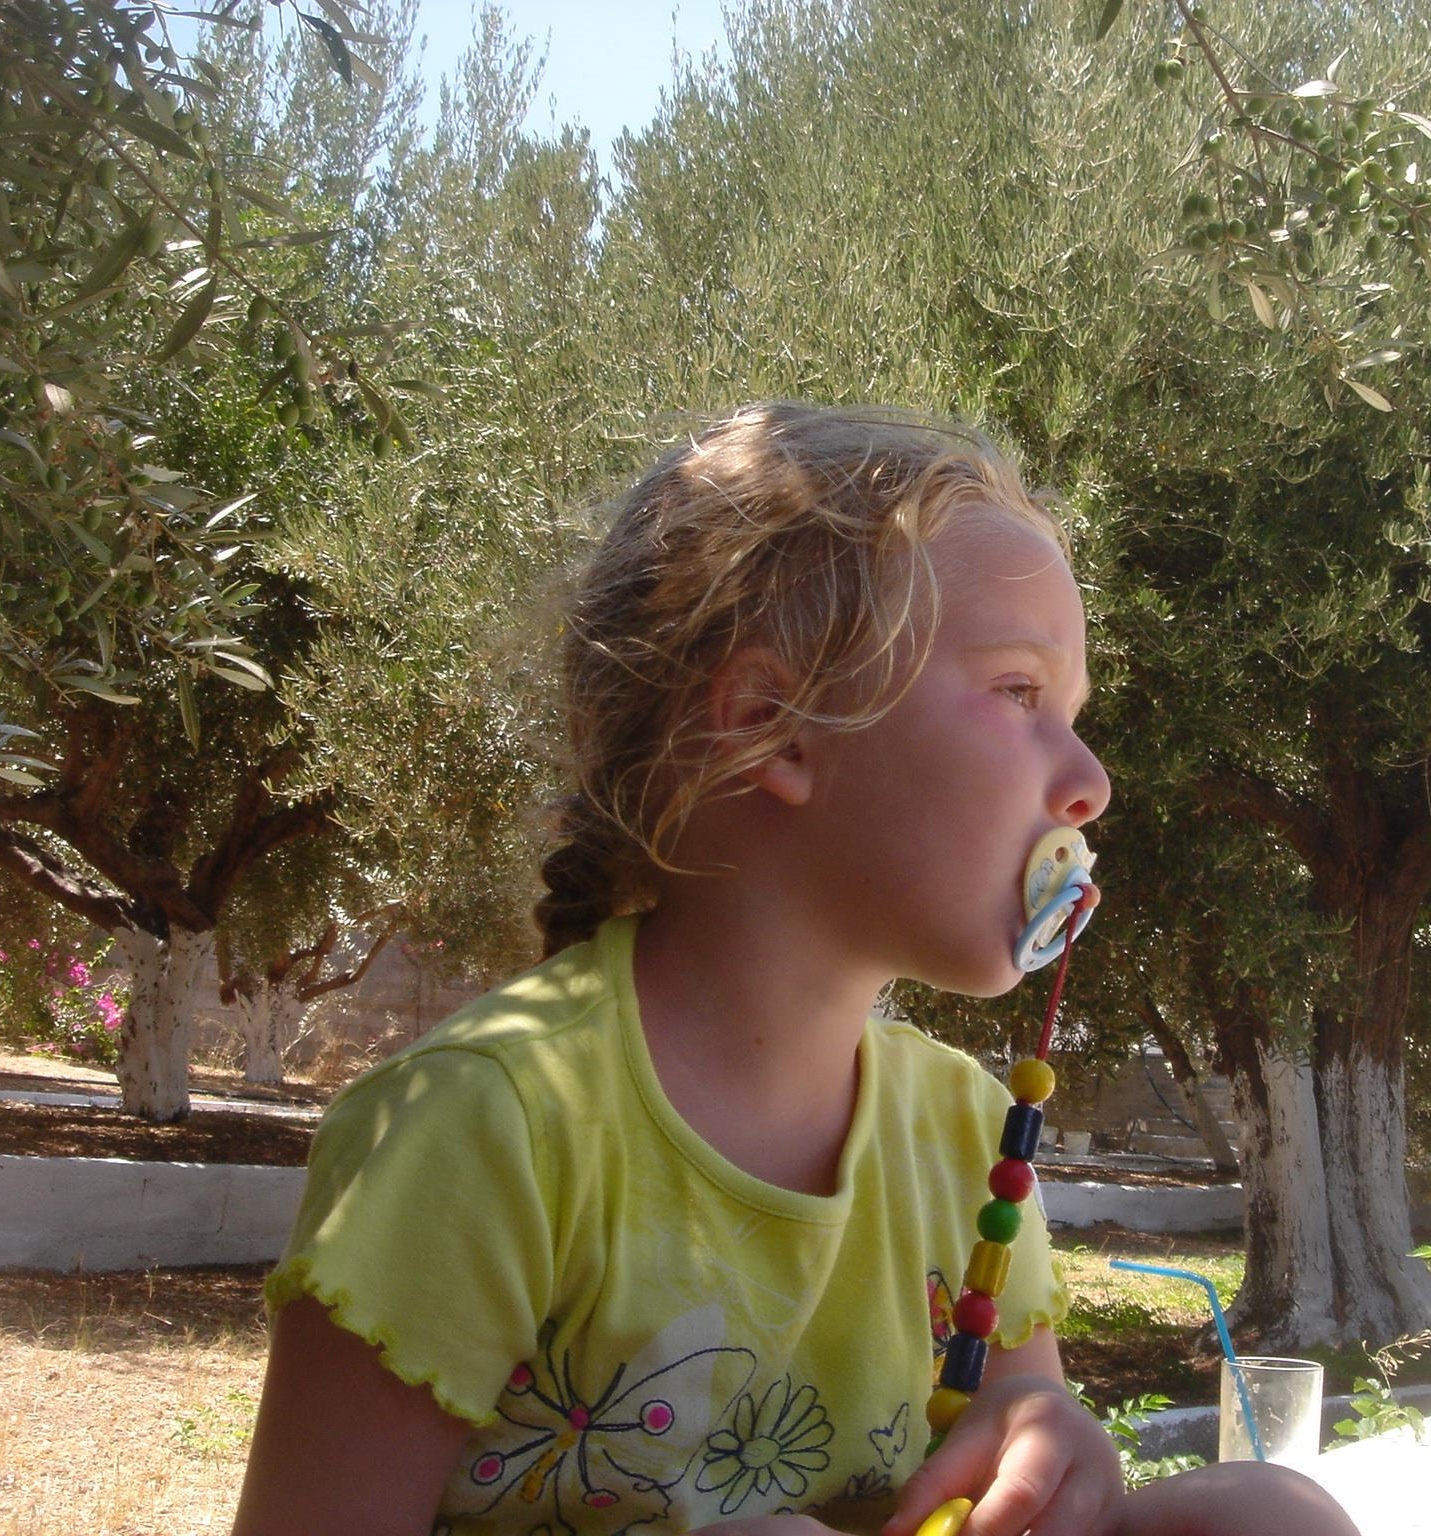
\includegraphics[width=\textwidth]{images/chapter3.jpg}
\end{figure}
\begin{minipage}[c]{\textwidth}
\recette{Sauce vinaigrette}
\ingredients{
\item Huile. 
\item 1 cuillère à café de moutarde.
\item 1 bonne cuillère à soupe de vinaigre.
}
Mélanger le tout en battant énergiquement pour obtenir plus ou moins la même consistance qu’une mayonnaise.\\
\\

\end{minipage}

\begin{minipage}[c]{\textwidth}
\recette{Sauce béarnaise}
\ingredients{
\item 2 jaunes d’œufs
\item 2 cuillères à soupe de sauce (quelle sauce ?) 
\item 1 pincée de sel. 
}
Mélanger le tout à l’aide d’un fouet. Cuire à feu doux en tournant toujours (ne pas laisser bouillir !). Ajouter du beurre par petits morceaux tout en fouettant.\\
\\

\end{minipage}

\begin{minipage}[c]{\textwidth}
\recette{Sauce blanche pour légumes}
Fondre du beurre.\\
Y ajouter $\nicefrac{1}{2}$ cuillère à soupe de farine et une pincée de sel.\\
Sur feu doux ajouter du lait en tournant. \\
Y Verser les légumes cuits à l’eau.\\
\\
NB : pour les épinards ajouter 1 cuillère à soupe de farine en plus pour allonger le légume. \\
\\

\end{minipage}

\begin{minipage}[c]{\textwidth}
\recette{Sauce mousseline (artichauts)}
Faire fondre au bain-marie 150 gr de beurre.\\
Faire réduire de moitié 4 cuillères à soupe de vinaigre.\\
Laisser tiédir.\\
Ajouter 2 jaunes d’œufs en fouettant.\\
Ajouter peu à peu le beurre fondu en fouettant toujours. \\
Saler.\\
Ajouter un peu de jus de citron.\\
Ajouter le reste du beurre.\\
Garder au chaud au bain-marie.\\
\\

\end{minipage}

\begin{minipage}[c]{\textwidth}
\recette{Sauce hollandaise (asperges) }
Mettre dans un poêlon $\nicefrac{1}{2}$ cuillère à soupe d’eau, 1 forte pincée de sel, le jus d’$\nicefrac{1}{2}$ citron (environ 1 cuillère à soupe) et 1 jaune d’œuf. \\
Mélanger alors seulement au fouet.\\
Mettre à feu doux en mélangeant au fouet jusqu’à début d’épaississement.\\
Incorporer peu à peu 60 gr de beurre en mélangeant bien, à très petit feu. \\
Mélanger sans arrêt.\\
\\
NB : Ne pas verser  la sauce dans une saucière plus chaude que la sauce.\\
\\

\end{minipage}

\begin{minipage}[c]{\textwidth}
\recette{Fines herbes}
Mélanger un peu de cressonnette, du persil, du cerfeuil, quelques feuilles d'épinard et d’oseille, 1 ou 2 petits oignons et 1 ou 2 feuilles d’artichaut (sans la partie blanche). Le tout doit peser environ 25 gr.\\
Hacher fin.  \\
\\
Peut s'employer par exemple en mélangeant les fines herbes à de la mayonnaise et en versant le mélange sur de la tête de veau (environ 150 gr par personnes) coupée en cube.\\
\\

\end{minipage}

\begin{minipage}[c]{\textwidth}
\recette{Sauce tartare}
\ingredients{
\item $\nicefrac{1}{4}$ L de mayonnaise
\item 1 gros oignon haché fin
\item 15 gr de feuilles d’estragon frais au vinaigre hachées finement
\item 1 cuillère à dessert de sauce anglaise
\item 25 gr de cornichons hachés 
\item 1 cuillère à dessert câpres hachées
\item Poivre et sel
\item $\nicefrac{1}{2}$ cuillère à café de vinaigre à l’estragon 
\item 1 cuillère à café de moutarde
}
Mélanger au fouet et servir bien frais ! \\
\\

\end{minipage}

\begin{minipage}[c]{\textwidth}
\recette{Ketchup aux pommes}
Prendre 12 pommes pelées, vidées et découpées en quartier. Les couvrir d'eau et laisser mijoter jusqu'a ce qu'elles deviennent molles, passer le tout, ajouter par litre de pomme :\\
une tasse de sucre\\
une cuillère à thé de moutarde\\
une cuillère à soupe de sel\\
une cuillère à thé de clous de girofles\\
2 cuillère à thé de canelle\\
2 tasses de vinaigre de cidre\\
2 oignions râpés\\
Laisser mijoter pendant une heure. Mettre en bouteille.\\
\\

\end{minipage}




\chapter{Désserts}
\begin{figure}[h]
\centering
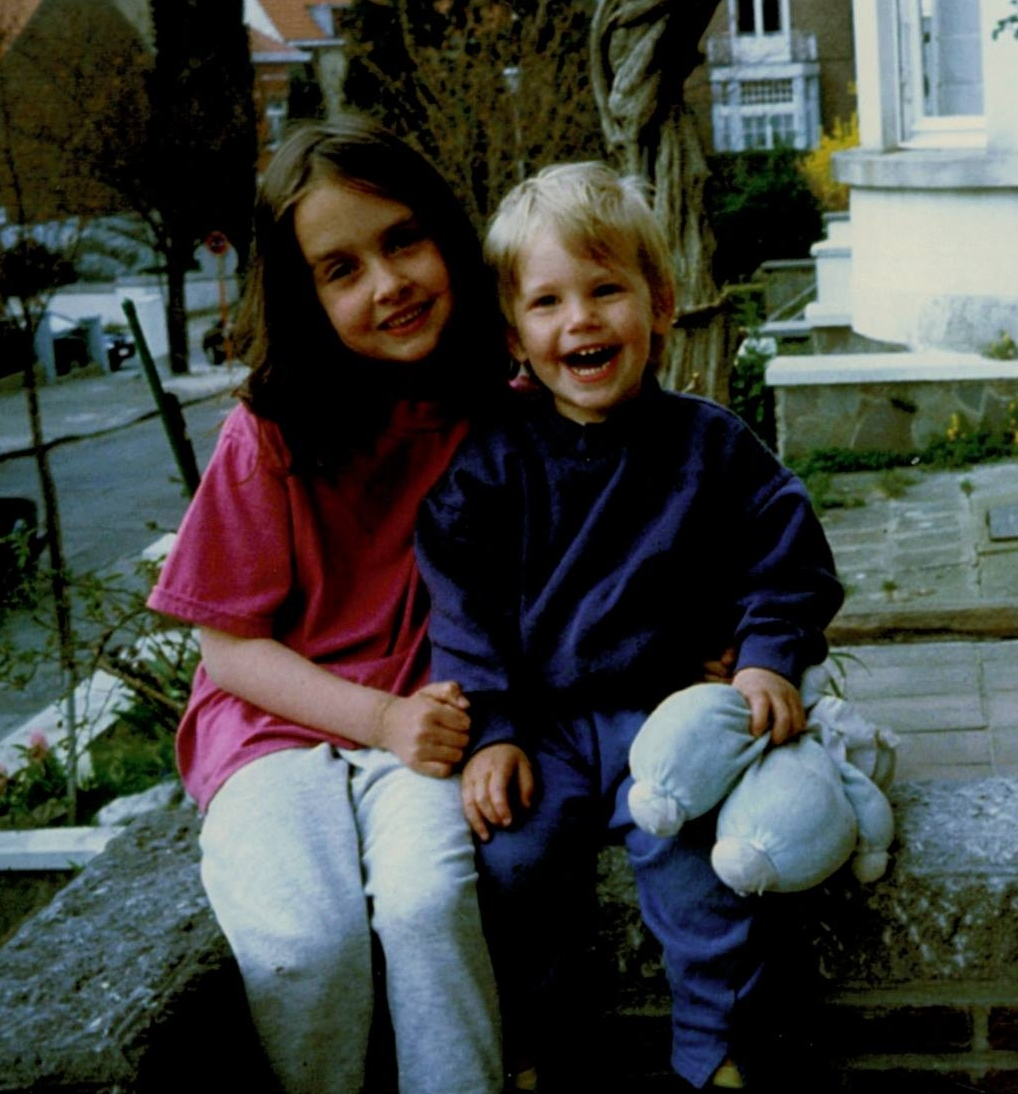
\includegraphics[width=\textwidth]{images/chapter4.jpg}
\end{figure}
\begin{minipage}[c]{\textwidth}
\recette{Puits d’amour }
\ingredients[(par personne)]{
\item 1 blanc d’œuf en neige + 1 cuillère à soupe de sucre. 
\item 1 jaune + 1 cuillère à soupe de sucre. 
}
Mélanger au fouet jusqu’à ce que ca cloque. Verser le jaune dans le fond du bol. \\
Ajouter une cuillère à café de cognac ou de rhum et/ou une cuillère à café de gelée de groseille. \\
Ajouter le blanc en neige. \\
Un peu de gelée de groseille au sommet. \\
Chacun mélange dans son bol à table !\\
\\

\end{minipage}

\begin{minipage}[c]{\textwidth}
\recette{Äpfel auf der Schuëssel}
Peler les pommes et couper la pomme vidée en 2 krizt ?\\
Beurrer le moule et le mettre au four. Y mettre les pommes + un morceau de beurre, et « un rien » d’eau. \\
Sucrer. \\
Cuire +- 10 minutes. \\
Retirer du four et combler les trous avec de la confiture. \\
Battre 2-3 jaunes d’œufs avec du sucre et de la farine (très peu). Ajouter un zeste de citron. \\
En faire une crème.  \\
Battre les blancs en neige. \\
Mélanger, puis verser le tout sur les pommes. \\
Remettre à feu doux 10 à 15 minutes. \\
\\

\end{minipage}

\begin{minipage}[c]{\textwidth}
\recette{Crème d’amande }
Piller 100g d’amandes avec 100g de sucre. Ajouter 40g de beurre ramolli, deux jaunes d’œufs et deux cuillères de Rhum. Bien mélanger à la spatule. Utiliser sans cuisson.\\
\\

\end{minipage}

\begin{minipage}[c]{\textwidth}
\recette{Purée de châtaignes}
Laver les châtaignes. Les fendre tout autour pour couper les 2 peaux. \\
Jeter dans l’eau bouillante et faites repartir très rapidement l’ébullition. \\
Quand les deux peaux sont ouvertes (3 à 4 minutes), les égoutter, et couvrir pour que l’eau ne s’évapore pas et finir d’éplucher. \\
Jeter les châtaignes épluchées dans l’eau bouillante. Faire repartir l’ébullition mais la régler lentement. \\
Après 15 à 20 minutes d’ébullition (quand une dent de fourchette peut y pénétrer), égoutter au max. \\
Ne pas cuire trop longtemps. Si il y a un peu trop d’eau, ca empêche d’avoir une purée sèche…\\
Ecraser au moulin-légumes 3 fois de suite avec grilles de plus en plus fine : ca donne de la purée. \\
! La purée à manger telle quelle peut être faite au lait !\\
\\

\end{minipage}

\begin{minipage}[c]{\textwidth}
\recette{Petites poires en châtaignes}
\ingredients{
\item 1 kg  de purée sèche de châtaignes (recette précédente) 
\item 100 gr de sucre
\item 30/40 kg de beurre
\item 100 gr de choco râpé 
\item 1 jaune d’œuf
\item 50 gr d’angélique 
}
Mélanger la purée, le sucre, le jaune d œuf et le beurre. \\
Faire de ce mélange des boulettes très sucrées qu’on moule en forme de poires. \\
Rouler celles-ci dans le chocó rapé. \\
Piquer le bâtonnet d’angélique en queue.\\
\\

\end{minipage}

\begin{minipage}[c]{\textwidth}
\recette{Mousse de pommes }
\ingredients[(6 à 8 personnes)]{
\item Pommes reinettes : 1,2 kg
\item Sucre en poudre : 150 gr
\item Gélatine : 7 feuilles
\item Eau chaude : 1 cuillère a soupe
\item Pour le caramel : sucre (100-150 gr) et une cuillère à soupe d’eau.
}
Eplucher les pommes, retirer les pépins. Faire de la compote et y ajouter 150 gr de sucre. \\
Cuire 10 minutes. \\
Tremper la gélatine 10 à 15 minutes dans de l’eau froide. \\
Ajouter dans la casserole à une cuillère à soupe d’eau chaude, les feuilles de gélatine une à une en tournant à la spatule. \\
Passer la compote et la verser dans une terrine. Y ajouter la gélatine délayée et battre vigoureusement au fouet 15 à 20 minutes. \\
Ca donne un mélange ferme et blanc neigeux. \\
Verser dans un moule à charlotte caramélisé ou dresser en dôme dans une patte foncée avec une spatule trempée d’eau chaude. \\
Faire un caramel dans un poêlon. Quand il atteint la teinte recherchée, y ajouter $\nicefrac{1}{2}$ verre d’eau. Reprendre l’ébullition du caramel, sinon la mixture sera trop épaisse.\\
En verser un peu sur le dôme de compote obtenu et servir le reste dans une saucière.\\
\\

\end{minipage}

\begin{minipage}[c]{\textwidth}
\recette{Princesse cake }
\otor{Tilou}
\ingredients{
\item 6 cuillères de farine
\item 6 cuillères de sucre
\item 6 cuillères de lait
\item 2 œufs entiers
\item 125 de beurre ramolli
}
Cuisson : 20 minutes à four moyen\\
\\

\end{minipage}

\begin{minipage}[c]{\textwidth}
\recette{Petits four aux blancs d’œufs}
\ingredients{
\item 30 à 40 petits fours.
\item 2 blancs d’œufs
\item 90 gr de sucre en poudre 
\item Un zeste de citron râpé finement
}
Mélanger le tout au batteur (blancs non battus en neige à l’avance).\\
Huiler une feuille de papier blanc, poser sur une tôle, en grosses gouttes (1/2 noix). \\
Y laisser anuber le mélange à 3 minutes d’intervalles\\
Cuire à four doux 15 à 20 minutes. Découler du papier et conserver dans une boite en fer.\\
\\

\end{minipage}

\begin{minipage}[c]{\textwidth}
\recette{Crème à la glace }
\otor{Odette}
\ingredients{
\item 1 boule de lait « évaporé »
\item 2 cuillères de sucre fariné
\item 2 jaunes d’œufs
\item OU
\item 1 boite de lait condensé 
\item 1/3 tiers de lait (grandeur de la boite de lait évaporé)
\item 2 jaunes d’œufs 
\item Ajouter crème fraiche à volonté 
}
Parfums : \\
2 cuillères à soupe de Nescafé \\
2 cuillères à soupe de confiture\\
Sucre vanillé\\
\\

\end{minipage}

\begin{minipage}[c]{\textwidth}
\recette{Flan caramel}
1. Confection du caramel :\\
Chauffer 6 cuillères à soupe de sucre et $\nicefrac{1}{2}$ verre d’eau à feu vif. \\
Remuer jusqu’à ce que la mousse soit très blonde. \\
Verser alors dans le flotter terre et l’étendre en tournant\\
2. Battre 5 œufs entiers avec 5 cuillères à soupe de sucre. \\
Faire bouillir $\nicefrac{3}{4}$ d’une pinte de lait, puis y verser les œufs.\\
3. Verser le tout sur le caramel\\
4. Cuire à four chaud, baissé à $\nicefrac{1}{2}$ dans la plaque + eau bouillante pendant 25 minutes !\\
\\

\end{minipage}

\begin{minipage}[c]{\textwidth}
\recette{Dartois à la crème d’amande }
Etaler 2 rectangles de pâtes feuilletés (30 cm x 10-12 cm). L’un des rectangles mince, l’autre le double de volume.\\
Poser la bande mince sur la toile à pâtisserie, étaler une bonne couche de crème d’amande (recette précédente), humecter les bords à l’eau froide et y coller la deuxième bande de pâte. \\
Pour la deuxième bande de pâte, boucher les bords avec les doigts. \\
Dorer à l’œuf. Rayer avec la pointe d’un couteau et piquer avec l’aiguille sur toute l’épaisseur. \\
Cuire au four 20 à 30 min.\\
Saupoudrer de sucre glace et doré au four quelques minutes (surveiller)\\
\\

\end{minipage}

\begin{minipage}[c]{\textwidth}
\recette{Le phare du Finistère}
Mélanger 250g de sucre en poudre à 4 œufs entiers. Délayer avec un Litre de lait chaud.  Ajouter 125 g de raisins et 1 verre à liqueur de Rhum. \\
Enfourner dans un plat bien beurré environ 1 heure. \\
A manger chaud ou froid !\\
\\

\end{minipage}

\begin{minipage}[c]{\textwidth}
\recette{Strudel}
\ingredients{
\item Pâte : 
\item 250 g de farine
\item 1 œuf
\item 2 cuillères à soupe d’huile
\item Quelques cuillerées de lait
\item 1 cuillère à café de sel
\item Garniture :
\item 1 kg de pomme
\item 150g de sucre
\item 100g de beurre
\item 100g de chapelure brune
\item 50g de raisins secs
\item 50g d’amandes
\item 1 cuillère à soupe de cannelle en poudre
}
1. La pâte\\
Dans la terrine en fontaine, mettre la farine, le sel, l’huile et l’œuf. Travailler avec les doigts en ajoutant peu à peu le lait pour avoir une pâte mole. Travailler cette dernière 10 minutes avec la paume de la main jusqu’à ce qu’elle soit bien unie. \\
En faire une boule et laisser reposer une heure dans un torchon humide. \\
2. La garniture\\
Peler et couper les pommes en tranches  (plutôt petites lamelles).\\
Les mettre dans une terrine avec environ $\nicefrac{1}{2}$ sucre (75g), y faire fondre le beurre et y ajouter la chapelure. \\
Remuer quelques instants avec la cuillère en bois. Tout le beurre doit être absorbé. \\
Garder un peu au chaud. \\
Nettoyer les raisins et les gonfler dans un peu d’eau chaude. \\
3. Etendre la pate d’abord au rouleau puis l’étirer sur un drap jusqu’à ce qu’elle soit très fine, en badigeonnant au pinceau trempé dans de l’huile pour éviter qu’elle sèche ou casse. Obtenir une grande surface, environ 1m carré très fine comme du papier. \\
Mettre des pommes à une des extrémités. \\
Saupoudrer de chapelure cuite et de beurre puis de raisons, d’amandes et de cannelle et le reste du sucre.\\
Prendre la pâte dans les deux mains au dessous et faire rouler la garniture jusqu’au bout. On a fait ainsi un grand chausson. \\
Dorer à l’œuf (jaune) et glisser à four chaud sur la plaque à pâtisserie environ $\nicefrac{1}{2}$ heure. \\
Trois minutes avant la fin, saupoudrer de sucre et faire caraméliser en surveillant car cela brûle très vite ! A servir chaud, tiède ou froid.\\
\\

\end{minipage}

\begin{minipage}[c]{\textwidth}
\recette{Tuiles }
\ingredients[(pour 4 personnes)]{
\item 100 gr de beurre fondu
\item 100 gr de sucre glace
\item 5 cuillerées à soupe de jus d’orange
\item 1 cuillerée de Grand Marnier
\item 100 gr d’amandes effilées
\item 30 gr de farine
\item Le zeste râpé d’une orange
\item 1 pincée de sel
}
Mélanger beurre, sucre et le zeste d’orange, puis incorporer le jus d’orange et le Grand Marnier. Ajouter la farine et le sel. \\
Laisser reposer 2 heures au frigo. \\
Allumer le four à thermostat 5 (environ 150 degrés). Sur une plaque anti adhésive ou du papier sulfurisé, disposer de petits tas de pâte. Les étaler avec les doigts pour leur donner une forme ovale, puis les parsemer d’amandes. \\
Faire cuire au four et retirez dès que la pâte blondit. Laisser tiédir. \\
Décoller les tuiles avec une spatule et les disposer sur un rouleau à pâtisserie ou une bouteille en verre. \\
Laisser refroidir, garder au frais dans un endroit sec. \\
Servir avec les oranges (ci dessous)\\
\\

\end{minipage}

\begin{minipage}[c]{\textwidth}
\recette{Salade d’oranges }
\otor{Vivette}
Couper à vif une orange par personne en fines tranches. \\
Faire un sirop de sucre : environ 100 gr de sucre et 2 cuillères à soupe d’eau sur feu doux en tournant très souvent. Aromatiser avec de la badiane (ou anis étoilé). \\
Verser sur les oranges.\\
\\

\end{minipage}

\begin{minipage}[c]{\textwidth}
\recette{Charlotte aux pommes}
\ingredients{
\item 800 gr de pommes
\item 400 gr de sucre
\item 3 verres à moutarde d’eau
\item 1 bâton de vanille
\item Le jus d’1 citron
\item Calvados
\item Boudoirs (« biscuits »)
\item Crème fraiche
}
Peler les pommes et enlever l’intérieur. Couper les morceaux. Ajouter 300 gr de sucre, les 3 verres à moutarde d’eau, le jus de citron et le bâton de vanille. Cuire le tout très doucement pendant 40 minutes. \\
Garder un verre d’eau. Y ajouter 100 gr de sucre et faire un sirop. Refroidir puis ajouter un décilitre de calvados. \\
Beurrer un moule à charlotte. Tremper les 36 biscuits à la cuillère dans le sirop et les ranger bien serrés dans le moule (fonds et bords). \\
Dans le fond, ajouter une couche de pomme et le reste du calvados, une couche de biscuits trempés, une couche de pomme, une couche de biscuits… jusqu’au dessus. \\
Poser une petite assiette avec un poids dessus. Mettre au frigo. \\
Garnir de crème fraiche avant de servir !\\
\\

\end{minipage}

\begin{minipage}[c]{\textwidth}
\recette{Gâteau aux pommes }
Peler et épépiner 250 gr de pommes. Cuire au beurre rapidement -> sucre (un peu). ?? Ajouter 40 gr de sucre, 40 gr de beurre, 1 jaune d’œuf, 60 gr de farine, $\nicefrac{1}{2}$ paquet de levure sèche et le blanc d’œuf battu en neige. Mélanger et parfumer avec des zestes d’orange ou de citron râpé. \\
Cuire 30 à 40 minutes dans une cocotte fermée et beurrée à four doux.\\
On met une cocotte dans le four ? \\
\\

\end{minipage}

\begin{minipage}[c]{\textwidth}
\recette{Truffe aux noisettes}
Prendre du chocolat (250 gr) râpé ou fondu doucement avec une cuillère d’eau et le mélanger avec 250 gr de sucre en poudre.\\
Griller et râper à la moulinette 250 gr de noisettes et mélanger au mélange choco et sucre. Ajouter 150 gr de beurre ramolli, 1 paquet de sucre vanillé. Si le mélange est trop épais, ajouter 1 ou 2 cuillères de lait. \\
Reposer au frais 1 à 2 heures. \\
Former des boules avec les mains et rouler dans le choco râpé ou granulé. \\
Conserver au frais jusqu’au moment de servir.\\
\\

\end{minipage}

\begin{minipage}[c]{\textwidth}
\recette{Truffe de l’ogre}
Passer à la moulinette 200 gr de biscuits à la cuillère. Y incorporer 250 gr de choco râpé, 200 gr d’amandes râpées, 200 gr de sucre fin, 250 gr de beurre mou, 2 jaunes d’œufs, 1 cuillère à café d’essence de café et 2 cuillères à dessert de whisky. \\
Former des boules et les rouler dans le choco râpé ou granulé. \\
Garder au frais jusqu’au moment de déguster. \\
\\

\end{minipage}

\begin{minipage}[c]{\textwidth}
\recette{Truffe au chocolat}
Mélanger 250 gr de beurre avec 125 gr de cacao. Malaxer avec une cuillère en bois. \\
Sirop : $\nicefrac{1}{2}$ cuillère de sucre et $\nicefrac{1}{2}$ verre d’eau. Cuire 7 à 10 minutes jusqu’à ce que ca devienne du sirop (une grosse goutte ronde). \\
Verser peu à peu le sirop de cacao et le beurre en remuant bien. Ajouter 2 petits verres de liqueur. Battre à la cuillère en bois.\\
Mettre au froid. \\
Faire des boules et les rouler dans le cacao. \\
\\

\end{minipage}

\begin{minipage}[c]{\textwidth}
\recette{Tarte alsacienne}
1. Prendre 500g de cerises rouges transparentes, les laver, enlever la queue et les noyaux.\\
2. Préparer la même crème que pour le clafoutis : deux œufs, une cuillère à café de farine, deux cuillères à soupe de sucre en poudre, 70 gr de crème épaisse (ou beurre), un verre de lait et un petit verre de kirsch.\\
3. Préparer une pâte brisée :\\
150 gr de farine, 80 gr de beurre, 1/3 de verre d'eau et une pincée de sel.\\
Malaxer du bout des doigts dans une terrine tout ces éléments jusqu’à obtenir une boule de pâte que l’on abaisse au rouleau à une épaisseur de 3 mm.\\
4. Garnir un moule à tarte beurré : Poser les cerise sur la pate, puis y verser la crème. Porter au four chaud pendant 35 minutes, puis laisser refroidir et démouler.\\
\\

\end{minipage}

\begin{minipage}[c]{\textwidth}
\recette{Tarte au Reine-Claude}
\ingredients{
\item 150 gr de farine
\item 75 gr de beurre
\item Un peu de lait
\item 1 cuillère à café de bicarbonate
\item 1 pincée de sel
\item 1 cuillère à soupe de sucre
}
Etendre la pâte à la main dans la platine, la piquer à la fourchette.\\
Y placer un livre de Reine-Claudes coupées, la tranche en l'air.\\
Sucrer à la sortie du four.\\
\\

\end{minipage}

\begin{minipage}[c]{\textwidth}
\recette{Crème caramel }
Faire bouillir le litre de lait avec 75 gr de sucre.\\
Ajouter au lait bouillant un caramel formé en ajoutant un filet d’eau à 100 gr de sucre et en l’ayant laissé cuire jusqu’à brunissement. \\
Ajouter 3 cuillerées de custard préalablement délayée à l’eau froide.\\
Laisser un peu refroidir dans le poêlon avant de verser dans un plat.\\
\\

\end{minipage}

\begin{minipage}[c]{\textwidth}
\recette{Tarte Normande }
\ingredients[(2 petites tartes)]{
\item 250 gr de farine. 
\item 1 œuf entier battu.
\item 15 gr de levure délayée dans de l’eau tiède.
\item 25 gr de sucre (environ 1 cuillerée à soupe)
\item 25 gr de beurre (environ 1 cuillerée à soupe)
}
Faire un puits avec la farine. \\
Mettre un peu de sel sur les bords du puits.\\
Mélanger le beurre et le sucre dans le trou du puits.\\
Ajouter l’œuf et la levure.\\
Pétrir jusqu’à obtenir une pâte lisse.\\
Diviser la pâte en deux et la laisser monter à chaleur douce le temps de la préparation de la garniture (fruits ou sucre + œuf battu et beurre).\\
Abaisser la pâte au rouleau. La mettre dans la platine graissée. La garnir.\\
Cuisson environ 20 minutes au four pas trop chaud.\\
\\

\end{minipage}

\begin{minipage}[c]{\textwidth}
\recette{Crème pâtissière}
Tourner en crème avec un fouet 3 jaunes d’œufs et 125 gr de sucre (environ 5 cuillerées) jusqu’à ce que ça « cloque » (environ 10 minutes).\\
D’autre part, délayer 3 cuillerées de maïzena avec un peu de lait froid.\\
Mélanger les deux préparations et verser les dans du lait bouillant en fouettant jusqu’à épaississement.\\
\\
Pour la crème à choux, fouetter la crème pâtissière jusqu’à refroidissement dans l’eau froide pour éviter les peaux.\\
\\

\end{minipage}

\begin{minipage}[c]{\textwidth}
\recette{Crêpes à la Paul Bouillard}
\ingredients{
\item 125 gr de farine.
\item 3 œufs battus au fouet.
\item 1 cuillerée de sucre.
\item 1 pincée de sel.
\item Du lait (à ajouter jusqu’à ce que la pâte soit bien liquide)
\item 1 forte cuillerée à soupe de beurre fondu.
\item 1 cuillerée de cognac, rhum ou kirsch (facultatif).
}
Mélanger le tout.\\
\\

\end{minipage}

\begin{minipage}[c]{\textwidth}
\recette{Fromage blanc en crème }
Bien battre 2 pots de fromage blanc.\\
Sucrer.\\
Ajouter 1 jaune d’œuf.\\
Mélanger et servir.\\
\\

\end{minipage}

\begin{minipage}[c]{\textwidth}
\recette{Pommes Bernoises}
Cuire les pommes de terre entières 5 minutes à l’eau bouillante.\\
Les égoutter et les passer à l’eau froide. \\
Saler.\\
Couper les pommes de terre en tranches et en garnir le fond d’un plat à gratin. \\
Ajouter du beurre fondu et couvrir de fromage (emmental ou gruyère) coupé en lamelles.\\
Cuire au four jusqu’à ce que ce soit doré.\\
\\

\end{minipage}

\begin{minipage}[c]{\textwidth}
\recette{Pâte feuilletée}
Faire un puits avec 250 gr de farine.\\
Ajouter 50 gr de margarine (environ $\nicefrac{1}{4}$ de paquet).\\
1 pincée de sel et de l’eau.\\
Mélanger la pâte en la travaillant d’abord du bout des doigts puis du poignet jusqu’à ce qu’elle soit bien lisse.\\
Rouler la pâte au rouleau à tarte, bien l’étendre.\\
Lui donner une forme rectangulaire. Encore bien la rouler. \\
La plier en trois dans les deux sens (-> 9).\\
La rouler au rouleau de nouveau. Lui redonner une forme rectangulaire.\\
Replier en 9.\\
La laisser reposer 15 minutes au froid.\\
Incorporer 50 gr de beurre ou de margarine.\\
Plier la pâte en 9 puis encore en 9. La plier en 9 puis encore en 9.\\
(On a finalement incorporé 200 gr de corps gras).\\
\\

\end{minipage}

\begin{minipage}[c]{\textwidth}
\recette{Wiener Torte }
\ingredients{
\item 100 gr de beurre.
\item 100 gr de chocolat râpé.
\item 100 gr de sucre.
\item 75 gr de chapelure blanche.
\item 5 œufs.
}
Dans une terrine, travailler le beurre déjà mou. \\
Ajouter le sucre, le chocolat. Travailler le tout à l’aide d’une spatule jusqu’à obtenir une mousse homogène. \\
Ajouter un à un les jaunes d’œufs. \\
Ajouter la chapelure.\\
Ajouter les blancs d’œufs battus en neige très ferme. \\
Beurrer un moule à tarte à bords hauts. Y poser dans le fond un papier beurré. \\
Verser la masser fluide.\\
Cuire à four doux 35 à 40 minutes. \\
\\

\end{minipage}

\begin{minipage}[c]{\textwidth}
\recette{Gâteau de 20 ans}
\ingredients{
\item 250 gr de chocolat râpé.
\item 250 gr de sucre en poudre.
\item 250 gr d’amandes épluchées.
\item 2 jaunes d’œufs.
\item 2 œufs entiers + 1 blanc d’œuf. 
}
Casser 2 œufs entiers dans une terrine.\\
Ajouter le sucre en poudre et mélanger à l’aide d’une spatule. \\
Ajouter le chocolat et mélanger.\\
Ajouter les amandes qui auront été préalablement jetées 1 minute dans de l’eau bouillante puis décortiquées et moulues.\\
Une fois que la pâte est homogène et épaisse, y incorporer en mélangeant à l’aide d’une fourchette les blancs battus en neige très ferme.\\
Verser la pâte dans un moule beurré avec un papier dans le fond.\\
Cuire à feu doux.\\
Laisser un peu reposer. \\
Détacher à l’aide d’un couteau.\\
\\

\end{minipage}

\begin{minipage}[c]{\textwidth}
\recette{Tourte Viennoise }
\otor{Tilou}
Casser 3 œufs en séparant les blancs des jaunes dans deux bols différents.\\
Ajouter 180 gr de sucre aux jaunes d'oeufs. Battre et jeter d’un seul coup 40 gr de farine. Ajouter une cuillerée à café d’eau. Fouetter encore 2 minutes.\\
Fouetter à part les blancs en neige ferme.\\
Mettre chauffer 180 gr de chocolat avec une cuillerée d’eau. Ajouter au chocolat fondu 180 gr de beurre.\\
Mélanger le mélange à base de chocolat à celui à base des jaunes d’œufs. \\
Ajouter les blancs en neige. \\
Verser le tout dans un moule beurré de 25 cm de diamètre et 5 cm de hauteur et enfourner dans un four très chaud en baissant la flamme de moitié.\\
Cuisson 25 minutes.\\
Défourner. Laisser le gâteau retomber. Le démouler après 30 minutes.\\
Ne manger que le lendemain. \\
\\

\end{minipage}

\begin{minipage}[c]{\textwidth}
\recette{Gâteau Anversois}
\ingredients{
\item 150 gr de farine.
\item 100 gr de fécule.
\item 200 gr de sucre.
\item 4 cuillerées de lait
\item 1 œuf (le blanc battu en neige). 
\item 100 gr de beurre tiède.
\item 30 gr de cacao en poudre.
\item 1 paquet de sucre vanillé.
\item 1 paquet de levure.
}
Mélanger le tout.\\
\\
Enfourner dans un four tempéré dans un moule à charnière beurré et avec un peu de farine.\\
\\
Glaçage :\\
Dans une casserole faire fondre au bain-marie 2 tablettes de chocolat. \\
1 bon morceau de beurre ($\nicefrac{1}{2}$ cuillère à soupe).\\
1 de sucre faune = 2 cuillères d’eau chaude ??\\
Bouillir.\\
Le mélange final doit être épais et mat.\\
Couler le mélange sur le gâteau.\\
\\

\end{minipage}

\begin{minipage}[c]{\textwidth}
\recette{Crème Anglaise}
Dans un bol battre 2 œufs, 2 cuillères à soupe de sucre, 20 gr de farine et un peu de lait ($\nicefrac{1}{2}$ cuillère à soupe).\\
Y verser un verre de lait (bouillant) parfumé soit avec de la vanille soit avec du cacao ou encore avec $\nicefrac{1}{2}$ cuillère à café d’essence de café et continuer à battre. \\
Verser le tout dans une casserole.\\
Un bouillon très bref.\\
Verser dans une terrine.\\
Laisser refroidir.\\
\\

\end{minipage}

\begin{minipage}[c]{\textwidth}
\recette{Crème Saint-Honoré}
Il suffit de verser dans la crème anglaise finie une feuille de gélatine fondue et battre 2 blancs d’œufs à ajouter au mélange avec une fourchette. Mettre le tout à refroidir.\\
\\

\end{minipage}

\begin{minipage}[c]{\textwidth}
\recette{Soufflé au pain}
Laisser tremper de la mie de pain dans du lait chaud. \\
Bien égoutter puis écraser à la fourchette.\\
Y mélanger 2 jaunes d’œufs, 100 gr de sucre en poudre et 100 gr de beurre fondu.\\
Battre 2 ou 3 blancs d’œufs en neige. L’incorporer à la préparation. \\
Verser le tout dans un plat beurré.\\
Mettre au four. Le soufflé doit devenir bien doré. \\
Servir chaud.\\
Napper de sauce abricot parfumée au kirsch (facultatif).\\
\\

\end{minipage}

\begin{minipage}[c]{\textwidth}
\recette{Crêpes}
\ingredients{
\item 600 gr de farine. 
\item 230 gr de beurre ou de margarine.
\item 4 œufs.
\item 100 gr de cassonade.
\item 100 gr de sucre blanc.
\item 1 litre de lait. 
}
Faire un puits avec la farine.\\
Ajouter une pincée de sel et les jaunes d’œufs. Mélanger avec une spatule.\\
Ajouter le beurre ou la margarine fondu.\\
Ajouter le lait.\\
Ajouter les blancs battus en neige.\\
Le résultat doit être une pâte liquide masquant le dos de la cuillère.\\
\\

\end{minipage}

\begin{minipage}[c]{\textwidth}
\recette{Riz dessert }
\ingredients[(2 personnes)]{
\item $\nicefrac{1}{2}$ litre de lait.
\item 75 gr de riz.
\item 1 ou 2 jaunes d’œufs.
\item 2 cuillères à soupe de sucre.
\item 1 morceau de beurre. 
}
Faire bouillir le lait. Y ajouter le riz.\\
Laisser cuire 30 minutes. \\
Ajouter le sucre, le jaune, le beurre et une goutte d’essence d’amande.\\
Garnir de geler de groseilles.\\
\\

\end{minipage}

\begin{minipage}[c]{\textwidth}
\recette{Bombe Marocaine}
Verser du riz dessert dans un bol beurré. \\
Laisser bien épaissir.\\
Pour démouler passer le bol au bain-marie.\\
Y verser un ?? au chocolat.\\
\\

\end{minipage}

\begin{minipage}[c]{\textwidth}
\recette{Glacé au chocolat}
Faire fondre une ?? de chocolat au bain-marie.\\
Y ajouter 1 cuillère à soupe d’eau chaude, $\nicefrac{1}{2}$ cuillère à soupe de sucre et 1 morceau de beurre.\\
Mélanger à feu vif.\\
Faire bouillir le mélange tout en tournant jusqu’à épaississement.\\
Verser sur la bombe.\\
\\

\end{minipage}

\begin{minipage}[c]{\textwidth}
\recette{Praliné}
\ingredients{
\item 50 gr d’amandes.
\item 60 gr de sucre farine. 
}
Mettre les amandes et le sucre dans un poêlon sur feu doux en mélangeant bien à la fourchette jusqu’à début d’épaississement. Attention à ne pas laisser bruler.\\
Une fois cuit, verser le mélange sur une plaque préalablement huilée. \\
Laisser refroidir.\\
Garder le praliné dans une boite en fer.\\
Avant de l’employer pour un gâteau ou tout autre dessert, le moudre avec un moulin.\\
\\

\end{minipage}

\begin{minipage}[c]{\textwidth}
\recette{Croute aux fraises}
Ajouter à la pâte ci-dessus expliquée deux œufs. \\
Mettre la pâte dans un moule. La cuire à part, sans la garnir de fruit, en couvrant d’un papier cuisson avec des pois.  \\
Garnir de fraises et de sucre au moment de servir.\\
\\

\end{minipage}

\begin{minipage}[c]{\textwidth}
\recette{Soufflé au Grand Marnier}
Pâte : Faire fondre 40 gr de beurre dans une casserole. Ajouter 40 gr de farine, un bon verre de lait et 40 gr de sucre. Tout en remuant la préparation au fouet, la porter à ébullition. Laisser tiédir.\\
Battre 5 jaunes d’œufs. Y incorporer les 5 blancs préalablement préalablement battus en neige bien ferme. Ajouter un petit verre de Grand Marnier. \\
Beurrer un moule. Le saupoudrer de sucre. Y mouler la pâte puis y verser le mélange œufs-Grand Marnier. Cuire à four modéré (max 200\degrees) pendant 25 minutes. \\
\\

\end{minipage}

\begin{minipage}[c]{\textwidth}
\recette{Tarte aux groseilles}
Pâte :\\
\\
250 gr de farine.\\
125 gr de beurre.\\
10 cl de lait.\\
$\nicefrac{1}{2}$ cuillère à café de bicarbonate.\\
\\
Faire un puits avec la farine. En son centre, y mettre tous les autres ingrédients. Ramener la farine avec deux doigts sur les autres ingrédients. Mélanger. \\
\\
Crème :\\
\\
2 œufs.\\
20 cl de lait.\\
100 gr de sucre.\\
1 cuillère à soupe de farine.\\
\\
Battre les deux œufs entiers. Ajouter la farine. Mélanger.\\
Faire bouillir le lait avec le sucre. Verser ce lait sucré sur le mélange œufs-farine.\\
Remettre le tout sur le feu. Fouetter jusqu’à l’obtention d’une crème relativement épaisse. Retirer du feu et laisser tiédir.\\
\\
Sur la pâte moulée dans le moule, étendre la crème. Garnir de fruits. \\
NB : Pour des groseilles rouges, les blanchir préalablement avec un peu de sucre.\\
\\
Mettre le tout au four (150 et 200\degrees). Cuisson entre 25 et 30 minutes.\\
\\

\end{minipage}

\begin{minipage}[c]{\textwidth}
\recette{Gâteau aux pommes (culte)}
250 gr de beurre\\
125 gr de sucre\\
Mélanger le tout. Ajouter 3 œufs entiers bien battus. \\
Verser par cuillérée 250 gr de farine et une cuillère à café de levure.\\
Verser la pâte dans un moule à cheminée préalablement beurré. Décorer de pommes découpées en quartier et tranchées (la partie ronde contre la cheminée) et cuire à feu doux.\\
\\

\end{minipage}

\begin{minipage}[c]{\textwidth}
\recette{Croute aux fraises (pâte croquante)}
\ingredients{
\item 250 gr de farine. 
\item 125 gr de sucre.
\item 1 œuf entier et 1 jaune d’œuf.
\item 1 pincée de sel.
\item 200 gr de beurre ramolli.
}
Faire une fontaine avec la farine. Mettre le beurre en son centre. L’incorporer à la farine avec deux doigts. Ajouter les œufs puis le sucre. Mélanger jusqu’à l’obtention d’une pâte bien lisse. Bouler la pâte, la saupoudrer de farine. Laisser reposer 15 minutes. \\
Mouler mince la pâte. Couvrir la pâte de papier cuisson avec des pois. Cuire à feu doux (125 – 150\degrees), la chaleur doit venir du dessus, pendant 20 – 25 minutes en surveillant bien. \\
Enlever les pois. \\
Pour dorer le dessus de la pâte, cuire pendant 5 minutes supplémentaires, la chaleur doit toujours venir du dessus.\\
Pour que la pâte soit bien croquante, la faire un jour à l’avance. La garder au frais. Le lendemain, avant de servir, la garnir de fraises et de sucre.\\
\\

\end{minipage}

\begin{minipage}[c]{\textwidth}
\recette{Clafoutis aux cerises}
1 kg de cerises rouges transparentes lavées, dénoyautées et équeutées. Les mettre dans un plat en terre préalablement beurré. \\
Dans une terrine à part, battre 2 œufs entiers et 1 jaune. Ajouter et mélanger une cuillère à soupe de farine. Ajouter et mélanger 150 gr de sucre en poudre. Ajouter et mélanger un bon morceau de beurre. Ajouter et mélanger un verre de lait et une pincée de sel. \\
Verser la préparation sur les cerises. \\
Préchauffer le four à 250\degrees. En enfournant, baisser la température de moitié. Laisser cuire jusqu’à ce que la crème se soit solidifiée (au moins 30 minutes).  \\
Sortir le plat du four et le saupoudrer de sucre.\\
Laisser refroidir avant de servir.\\
\\

\end{minipage}

\begin{minipage}[c]{\textwidth}
\recette{Soupe aux cerises}
\ingredients{
\item 1 kg de cerises noires pas trop grosses lavées et équeutées. Ne pas sortir les noyaux.
}
Dans une casserole, faire fondre 60 gr de beurre. Ajouter 1 cuillère à soupe de farine. Mélanger. Mouiller la préparation avec un verre de vin rouge et un verre d’eau. Mélanger et laisser bouillir. Ajouter les cerises quand ça bout. Réduire le feu et mélanger délicatement. Ajouter 3 cuillères à soupe de sucre en poudre et quelques pincées de cannelle. \\
Mettre le couvercle et laisser cuire à petit feu 20 minutes.\\
Ajouter deux petits verres de kirsch. Faire bouillir 3 minutes.\\
Sur le côté, faire frire dans du beurre des tranches de pain. Les mettre dans le fond de la soupière puis y verser les cerises. Servir chaud. \\
\\

\end{minipage}

\begin{minipage}[c]{\textwidth}
\recette{Gâteau 4/4 }
\ingredients{
\item 250 gr. de farine 
\item 250 gr. de sucre
\item 250 gr. de beurre
\item 250 gr. d’œufs (c'est-à-dire 4 œufs). Séparer les jaunes des blancs et battre ces derniers en neige. 
\item $\nicefrac{1}{2}$ paquet de levure.
}
Mélanger le tout et cuire à feu doux !\\
\\

\end{minipage}

\begin{minipage}[c]{\textwidth}
\recette{Brioche aux pommes}
Mélanger 250g de beurre avec 150g de sucre, puis 3 oeufs entiers bien battus. Versez alors 250 g de farine et 3 cuillères de lait et une cuillère à café de levure.  Déposez dans un moule à cheminée, glissez à four doux décoré de deux pommes coupées en quartiers et tranchées.\\
\\

\end{minipage}

\begin{minipage}[c]{\textwidth}
\recette{Gâteau Claude}
\ingredients{
\item Farine 250 gr.
\item Sucre 150 gr. 
\item 4 cuillères à soupe de lait froid .
\item Beurre tiède 100 gr. 
\item 250 gr. d’œufs (c'est-à-dire 4 oeufs). Séparer les jaunes des blancs et battre ces derniers en neige. 
\item $\nicefrac{1}{2}$ paquet de levure.
\item Une cuillerée de liqueur ou de sucre vanillé. 
\item Une poignée de raisins secs.
}
Cuire à four modéré.\\
\\

\end{minipage}

\begin{minipage}[c]{\textwidth}
\recette{Savoie}
Mélanger dans une terrine 250 gr. de sucre et 7 jaunes d’œufs. Garder les blancs pour plus tard.\\
Travailler avec le fouet en ajoutant un paquet de sucre vanillé, puis petit à petit, 100 gr de farine et 100 gr de fécule.\\
Battre en neige ferme $\nicefrac{1}{4}$ des 7 blancs d’œufs. Quand c’est un peu détendu, verser le reste des blancs avec souplesse. Mettre le mélange dans un moule beurré jusqu’au $\nicefrac{3}{4}$ de sa hauteur. \\
Cuire à feu très doux et régulier. Quand c’est cuit, laisser reposer dans le moule quelques minutes puis démouler sur une grille.\\
\\

\end{minipage}

\begin{minipage}[c]{\textwidth}
\recette{Beignets au platte kaas (fromage blanc)}
Mélanger 2 jaune d’œufs, 50 gr de sucre, 100 gr de farine et 250 gr de platte kaas.\\
Ajouter 2 blancs en neige ferme.\\
Mettre une cuillère à café à la fois dans la friture.	\\
\\

\end{minipage}

\begin{minipage}[c]{\textwidth}
\recette{Mousse au chocolat }
Faire fondre au bain marie une le chocolat. \\
Dans une terrine mélanger un jaune d’œufs avec une cuillère à soupe de sucre jusqu’à ce que ça cloque ! \\
Battre le blanc en neige ferme.\\
Incorporer 25 à 30 gr. de beurre au chocolat fondu.\\
Ajouter le jaune et le sucre au mélange.\\
Ajouter le blanc en neige avec une fourchette et l’incorporer légèrement pour ne pas briser le blanc. \\
Mixer le tout dans le bol.\\
\\

\end{minipage}

\begin{minipage}[c]{\textwidth}
\recette{Tarte aux reines-claudes}
\ingredients{
\item 150g de farine
\item 75g de beurre
\item un peu de lait
\item une cuillère à café de baking
\item une pincé de sel
\item une cuillère à soupe de sucre
\item un litre de reine claude
}
préparation :\\
Etendre la pâte à la main dans la platine et la piquer à la fourchette. Y placer les reines-claudes coupées la tranche en l'air. Mettre au four et sucrer à la sortie du four.\\
\\

\end{minipage}

\begin{minipage}[c]{\textwidth}
\recette{Kugelhopf alsacien}
Dans une terrine, travaillez 150g de beurre avec 150g de sucre et 6 jaune d'œufs jusqu'à ce que ce soit bien lisse. Incorporez y 180g de farine, 9 blancs d'oeufs en neige et les zeste d'un citron finement haché. Versez dans le moule à kugelhopf. Cuire à four chaud 3/4 d'heure. En sortant le gâteau du four, saupoudrez le de sucre en poudre et laissez le refroidir.\\
\\

\end{minipage}

\begin{minipage}[c]{\textwidth}
\recette{Tarte viennoise aux pommes}
Dans un récipient, verser 1/3 de verre d'eau froide et 160g de farine. Peu à peu, incorporer 80g de beurre, deux pincées de sel (si la pate colle un peu ajoutez y 1 cuillère de farine). En faire une boule que vous laissez reposer 1/4 d'heure dans une serviette. Roulez la pate et en garnir une platine beurrée. Piquez la pate avec une fourchette\\
La garnir de compote. Pour la compote : découper 150g de pomme du Canada et les mettre à cuire avec 4 cuillères de sucre .\\
Couper en quartier deux pommes crues et les disposer sur la compote.\\
Saupoudrer le tout d'une demie cuillère à café de cannelle, une cuillère de sucre et deux cuillère de farine. Enfourner 25 min\\
\\

\end{minipage}

\begin{minipage}[c]{\textwidth}
\recette{Tarte aux pruneaux}
La veille, tremper les pruneaux. Dénoyauter-les le lendemain\\
Faire une pâte à tarte avec 180g de farine, 90g de beurre, 1/3 de verre d'eau, 1 pincé de sel.\\
Couvrir la pâte mise dans la platine d'une crème faite avec deux jaunes d’œufs etun œuf entier, 4 cuillère de sucre et une de farine, 125g de crème, 1 verre de lait et 1 verre de kirsch.\\
Garnir de pruneaux ouverts. Cuire 35 à 40 min. Arrosez la tarte de kirsch chauffé et enflammer en servant\\
\\

\end{minipage}

\begin{minipage}[c]{\textwidth}
\recette{Puits d'amour}
Battre deux jaunes d'oeufs avec du sucre jusqu'a obtenir la consistance d'une mayonnaise. Remplir 5 moules du mélange, verser une cuillère de rhum et ajouter une couche de confiture de groseille et une couche de banc d'oeuf en neige sucré.\\
\\

\end{minipage}

\begin{minipage}[c]{\textwidth}
\recette{Soufflé à l'orange}
\ingredients{
\item trois oranges
\item 1 citron
\item 6 blancs d'œufs
\item 150g de sucre
}
Préparation : râper les zestes, battre les blancs en neige et y incorporer les zeste et le sucre.\\
Garnir un moule avec la préparation et y ajouter du sucre. Mettre 20 à 30 minutes à four doux.\\
servir le soufflé chaud.\\
\\

\end{minipage}

\begin{minipage}[c]{\textwidth}
\recette{Kugelhopf (bouillard)}
\ingredients{
\item 500g de farines
\item 200g de sucre
\item 12g de sel
\item 35g de levure
\item 3 oeufs
\item 200g de raisin sec
\item 150g de beurre
\item 1/10 de litre de lait
}
Faire un levain :\\
Mélangez la levure à 1/2 tasses à déjeuner de lait ou d'eau tiède. Versez au centre de la farine. Mélangez jusqu'à obtenir une pâte assez fluide. Recouvrir de farine et laisser monter jusqu'au rejet de la farine. Mélangez le restant de farine avec les oeufs, le sucre le sel et un peu de lait. Pétrissez et terminez par le levain. Mélangez le beurre et les raisins bien épongés. Mettez en moule pour le laisser monter. Enfournez comme le pain.\\
Cuire une heure au four à chaleur modérée.\\
\\

\end{minipage}

\begin{minipage}[c]{\textwidth}
\recette{Confiture d'orange}
Faire une julienne des zestes d'orange avec 6 oranges et 3 citrons épluchés très fins et coupés, le tout couvert de 3 L d'eau par kilo de fruit jusqu'au lendemain.\\
Faire alors évaporer le tiers et mettre par kilo restant 1200g de sucre. Faire cuire.\\
\\

\end{minipage}

\begin{minipage}[c]{\textwidth}
\recette{Salade de fruit}
\ingredients{
\item Deux oranges en tranche
\item Deux bananes en rondelle
\item 3 tranches d'ananas en dés
\item Une pomme
\item 10 amandes coupées en tranches
\item 1 cuillère de kirsch délayée dans une cuillère de gelé de groseille
\item Un jus de citron
}
Couvrir de crème fouettée et saupoudrer d'amande en tranche.\\
\\

\end{minipage}

\begin{minipage}[c]{\textwidth}
\recette{Beignet au pomme}
\ingredients{
\item 500g de farine
\item 3 oeufs
\item 100g de sucre (= 4 cuillères à soupe)
\item Une pincée de sel
\item Du lait
\item Une cuillère à soupe de levure
}
Incorporer les jaunes d'oeufs, le lait, le sel, la levure et le sucre à la farine jusqu'a obtenir une pate lisse. Ajouter légèrement les blancs en neige. Jeter sur la pate les rondelles de pommes au moment de mettre les beignets dans la friture bouillante.\\
Retourner avec une fourchette. Servir avec du sucre blanc.\\
\\

\end{minipage}

\begin{minipage}[c]{\textwidth}
\recette{Scones}
\ingredients{
\item 85 gr de margarine ou de beurre
\item 225gr de farine fermentante
\item 1 oeuf entier
\item 1 pincé de sel
\item Un peu de sucre
\item Raisins a volonté
}
Mélanger avec un peu de lait pour avoir une pâte a roulé puis couper en petite forme.\\
Cuisson a four chaud environ 20 min.\\
\\

\end{minipage}

\begin{minipage}[c]{\textwidth}
\recette{Confiture pomme au gingembre}
Peler et couper en quartier des pommes. Vider les et couper les en tranches assez épaisses. Ajouter pour un litre de pomme 3/4 de litre de sucre brun, 5 litres de jus, et des écorces râpées de 4 citrons, 250g de racines de gingembre ou de gingembre confit.\\
Laisser reposer 24h dans un bol. Bouillir jusqu'à ce que les pommes soit claires et aient une riche couleur d'ambre.\\
\\

\end{minipage}

\begin{minipage}[c]{\textwidth}
\recette{Tranches d pommes et gingembres}
Couper en petits morceaux 4 kilo de pommes sucrées non pelées. Ajouter 2 kg de sucre et 250g de gingembre confit. Laisser reposer 24h. Ajouter  4 citrons coupées en morceaux sans les pépins. Cuire lentement 3h. Mettre en bocal + parafins.\\
\\

\end{minipage}

\begin{minipage}[c]{\textwidth}
\recette{Massepain }
\otor{Tilou}
\ingredients{
\item 250g de sucre farine
\item 250g d'amande moulue
\item 2 cuillère à soupe d'eau
\item 1 cuillère à soupe d'eau de fleur d'oranger
\item 1 pincé de sel
}
Un blanc d'œuf en neige\\
Au bain marie\\
Versez le sucre petit à petit à l'eau (par cuillerée)\\
Jusqu’a faire ?\\
Versez petit à petit la poudre d'amande et entre temps pour détendre, une cuillère de blanc d'œuf battue\\
\\

\end{minipage}

\begin{minipage}[c]{\textwidth}
\recette{Soufflé au grand marnier}
Bouillir doucement 1/2 litre de lait et 150g de sucre\\
Dans une autre casserole, fondre 150g de beurre\\
Versez 40g de maïzena\\
Mélanger\\
Y mettre petit à petit le lait sucré pour faire une crème épaisse\\
Hors du feu\\
Versez un grand verre de liqueur grand Marnier, 5 jaunes d'œufs\\
Bien travailler\\
Ajouter 8 blancs en neige\\
Cuire à four moyen, préalablement chauffé, 16 à 18 minutes\\
\\

\end{minipage}

\begin{minipage}[c]{\textwidth}
\recette{Gauffre chaude }
\otor{Bonne Maman}
Un œufs + 1 cuillères de sucre + 1.5 cuillère de farine\\
à multiplier autant de fois qu'on veut\\
+ Un quart de beurre fondu? + Un peu de cannelle\\
Blanc en neige\\
Pour gauffres croquante mettre un peu d'eau\\
Cuire tout de suite\\
\\

\end{minipage}

\begin{minipage}[c]{\textwidth}
\recette{Tarte aux prunes }
\otor{Robert Ville}
200g de farine fermanté\\
80g de beurre\\
Mélangée en fontaine 2 œufs puis 10g de sucre\\
Recouvrir de prune\\
Saupoudrez le mélange de cannelle plus de sucre farine\\
Cuire le tout\\
\\

\end{minipage}

\begin{minipage}[c]{\textwidth}
\recette{Gâteau de famille au petit beurre}
Travailler ensemble 60g de beurre + 1 cuillère à café de sucre semoule, et un jaune d'œuf\\
Battre le blanc en neige ferme et mélanger légèrement à la pate\\
Trempez légèrement 24 petits beurres dans du café fort tiède ou froid\\
Étende une couche de biscuit puis une couche de crème alternativement\\
Recouvrir le gâteau terminé de chocolat râpé, ne pas cuire, manger le lendemain\\
\\

\end{minipage}

\begin{minipage}[c]{\textwidth}
\recette{Madeleine}
\ingredients{
\item 200g de farine
\item 225g de sucre fin
\item 2 paquets de sucre vanillé
\item 250g de beurre ou de margarine
\item 4 œufs
}
Faire fondre doucement le beurre (sans le laisser cuire) et refroidir\\
Dans un grand bol mélanger au fouet les jaune d'œufs et le sucre jusqu'au ce que ça mousse\\
Ajouter le beur fondu puis la farine petit à petit, une cuillère à café de jus de citron, et les zeste râpé fins\\
Battre les blancs en neige ferme et ajouter à la pâte en les soulevant délicatement\\
Mettre au frigo 40 min\\
Beurrer au pinceau les moules avec du beurre fondu, fariné, remplir les moule à 2/3 de pate\\
Cuisson 10 à 20 minute à four moyennement chaud, démoulé sur grille.\\
\\

\end{minipage}

\begin{minipage}[c]{\textwidth}
\recette{Tarte aux raisins}
Pate sablé avec 250g de farine tamisé, 100g de sucre, une pincé de sel\\
Ajouter un à un 2 œufs entiers\\
Puis 70g de beurre en petit morceau\\
Mélanger rapidement\\
Laisser reposer une heure\\
Abaisser au rouleau\\
Mettre dans le moule à tarte bien beurrer\\
Remplir de raisin frais\\
Cuire à four chaud 15 min \\
Sucrer à la sortie du four\\
On peut aussi napper d'un appareil à meringue (blanc + sucre battu) et dorer au four\\
\\

\end{minipage}

\begin{minipage}[c]{\textwidth}
\recette{Tarte frangipane}
Mélanger 150g d'amande douce, 100g d'amande amer avec un peu de lait\\
Ajouter 500g de sucre en poudre et 1/2 l de lait\\
Dans un bol mélanger à la spatule 250g de beurre\\
250g de sucre puis 5 jaune d'œuf entier un par un et 150g de farine\\
Mélanger les 2 pates\\
Cuire dans une platine à tarte à four chaud\\
\\

\end{minipage}

\begin{minipage}[c]{\textwidth}
\recette{Gâteau marrons noël (excellent !!)}
1 kilo 250 de pate de marrons glacé (ou de crème de marron un peu séchée à four très doux)\\
Et des marrons entier moulus\\
Incorporez 100g de beurre ramolli et une petite cuillerée de kirsch ou de cognac\\
Bien mélanger à la spatule en bois, laisser reposer au frais\\
Ensuite dans une terrine, versez et mélangez, 250g d'amande moulue, 150g de sucre en poudre, 150g de beurre, 2 jaune d'œuf, 3 cuillère à soupe d'extrait de café\\
Tapissé un moule à charlotte de 18cm de diamètre d'une mousseline (étamine à frittes) qui doit déborder largement\\
Tasser dans le fond la moitié de la pâte de marron au-dessus la pâte d'amande et couvrir avec la pâte de marron\\
Rabattre la mousseline sur le dessus du gâteau\\
Y poser une assiette avec un poids dessus, mettre au frigo une nuit, démouler le lendemain en tirant doucement l'étame\\
Glaçage:\\
    Faire fondre à feu doux 250g de chocolat, 2 cuillère à café d'eau, 2 cuillère à café d'extrait de café\\
    Remuer à la spatule jusqu'à obtenir une pate lisse\\
    Ajouter 50g de beurre,\\
    Mélangez\\
Trempez une spatule en métal dans de l'eau bouillante et l'utiliser pour lisser la crème au chocolat sur le gâteau et les coté\\
Garnir avec des demi-noix, des cerises confite ou des feuilles de houx\\
\\

\end{minipage}

\begin{minipage}[c]{\textwidth}
\recette{Gâteau à la noix de Cosette }
Ramollir 100g de beurre\\
Incorporer 200g de sucre\\
Battre a fouet jusqu'à ce que ça devienne blanc et mousseux\\
Incorporer peu à peu 200g de poudre de noix puis 4 jaune d'œuf un à un\\
Battre le balcon en neige très ferme\\
Les incorporer délicatement au mélange\\
Beurrer un moule à ? De 20 à 23 cm de diamètre\\
Cuire à four chaud 30 à 35 minute (jusqu'à ce qu'une aiguille piquée au milieu ressorte sèche, éventuellement couvrir d'un papier d'argent en fin de cuisson pour éviter de bruler)\\
Laisser refroidir dans le four éteint\\
Peut-être décoré de crème chantilly et de noix mais c'est déjà assez nourrissant\\
\\

\end{minipage}

\begin{minipage}[c]{\textwidth}
\recette{Spéculoos }
\otor{Catherine}
\ingredients{
\item 200g de farine
\item 175g de cassonade
\item 125g de beurre
\item 1/2 cuillère à café de cannelle
\item 1/2 cuillère à café de levure en poudre
\item 1/2 cuillère à café de bicarbonate de soude
\item 1 œuf
}
Tout mélanger\\
Laisser reposer une nuit au frais\\
Aplatir au rouleau,\\
Mettre dans le moule,\\
Cuisson 15 min à feu moyen\\
nb: les spéculoos sont mou à la sortie du four mais ils durcissent en se refroidissant\\
\\

\end{minipage}

\begin{minipage}[c]{\textwidth}
\recette{Crème anglaise }
\otor{Tilou}
Battre au fouet 2 jaune + 2 cuillère à soupe de sucre jusqu'à ce que ça blanchisse\\
Ajouter une cuillère à soupe rasé de farine (20g)\\
Délayer dans un peu de lait\\
Versez un grand verre de lait chaud (250ml) en tournant\\
Faire bouillir sur le feu,\\
Parfumez avec de la vanille, du cacao ou du café\\
Laisser refroidir en tournant de temps en temps pour éviter la peau\\
\\

\end{minipage}

\begin{minipage}[c]{\textwidth}
\recette{Gâteau sec }
\otor{Tilou}
\ingredients{
\item 3oeuf
\item 150g de sucre
\item 3 à 4 cuillère à soupe d'eau
\item 1 cuillère à soupe de jus de citron
\item 100g de farine
\item 100 de maïzena
\item 1 petit paquet de baking
}
Mélanger le jaune le sucre l'eau et le citron\\
Incorporer petit à petit la farine la maïzena le baking en alternant\\
Ajouter les blancs en neige\\
On peut ajouter avant les blancs 75g de beurre fondu et tiède\\
Cuisson 20 à 30 in à feu doux\\
\\

\end{minipage}

\begin{minipage}[c]{\textwidth}
\recette{Rombosses}
\ingredients{
\item 1 tasse de farine
\item 1/2 cuillère à café de sel
\item 1/3 tasse d'eau ou lait
\item 2 cuillères à café de baking
\item 2 cuillères à soupe de graisse
\item 4 pommes
\item 1/2 tasse de sucre
}
Faire une pâte molle et l'étendre au rouleau, la couper en forme carré, y mettre les pommes pelées et vider.\\
Remplir avec le sucre et la cannelle.\\
Mouiller les bords et en recouvrir la pomme. Percer à la fourchette pour laisser sortir la vapeur.\\
Cuire au four ou à la vapeur, la pomme doit être tendre. Servir avec du sucre et de la crème ou du sucre au citron. \\
\\

\end{minipage}

\begin{minipage}[c]{\textwidth}
\recette{Betty brune}
\ingredients{
\item 1 tasse de mie de pain
\item 8 pommes tranchées
\item 1 tasse de sucre
\item 1/2 tasse eau froide
}
Beurrer un plat allant au four et y mettre 1 couche de mie de pain, une couche de pomme, cannelle, sucre et beurre. Répéter jusqu'à ce que le plat soit rempli. Piquer avec 1 couteau pointu  et y verser l'eau et le sucre couverts du sirop. Faire cuire au bain marie 45 min. servir chaud avec de la crème.\\
\\

\end{minipage}

\begin{minipage}[c]{\textwidth}
\recette{Tarte aux noix }
1\degrees faire une pâte sablée en travaillant du bout des doigts et rapidement. Laisser reposer 1h.\\
2\degrees rouler la pâte au rouleau ou l'abaisser à la main dans un moule d'un diamètre de 24 cm.\\
3\degrees melangez environ 250g de crème très fraiche, 100g de sucre en poudre, 100 g de noix moulues.\\
4\degrees garnir la pâte de ce mélange et cuire à four moyen pendant 30 min (surveiller)\\
5\degrees refroidir la tarte sur une grille\\
6\degrees glacer avec 1 mélange de 100g de sucre glace (=sucre farine) et 2 cuillères à soupe de kirsch. \\
Etendre cette pâte coulante sur la tarte à la spatule. Laissez sécher quelques heures.\\
\\

\end{minipage}

\begin{minipage}[c]{\textwidth}
\recette{Pommes au gingembre}
Couper les pommes en quartiers et tranches épaisses.  3/4 du poids de sucre brun clair par kg de pommes, 1 zeste de citron râpé, 100 g de gingembre confit par kg de pommes, 1 noix. Couper en morceaux, reposé 1 jour, bouillir jusqu'à ce que la couleur ambre jaune très clair.\\
\\

\end{minipage}

\begin{minipage}[c]{\textwidth}
\recette{Régal aux pommes (conserves)}
\ingredients{
\item 7 litres de pommes surgelées en cube
\item 1/2 litres de noix ou noix de pékan 
\item 3 litres de sucre
\item 2 oranges (écorce râpées et jus)
}
Mélanger et laisser reposer 1 nuit pommes-sucre-orange et raisins.\\
Cuire lentement 45 min en remuant  et à couvert jusqu'à ce que les peaux soient absorbés. Ajouter les noix 5 min avant d'enlever du feu. S’emploie avec les tartes, la viande, les beignets ou à conserver dans des bocaux.\\
\\

\end{minipage}

\begin{minipage}[c]{\textwidth}
\recette{Gâteau fruits confits}
Battre 2 œufs et 2 jaunes. \\
Ajouter 3 tasses de sucre semoule. Battre. \\
Ajouter 1 petite tasse de Corinthe (lavées)\\
Ajouter 1 petite tasse de raisins blancs (sultans)\\
Ajouter 50g de fruits confits. Coupés au rhum.\\
Ajouter écorces d'oranges confites\\
Ajouter 260 g de beurre ramolli\\
Ajouter 1 pincée de sel\\
Ajouter par cuillerées 4 tasses farine tamisée et 1 paquet de baking.\\
Ajouter des blancs d'œufs en neige. \\
Laisser reposer la  pâte 4h ou plus. Faire cuire 50 min dans une forme bien beurrée et farinée, remplir au 3/4.\\
\\

\end{minipage}



\backmatter
\pagestyle{empty}


\ifodd\thepage\hbox{}\newpage\else\fi%si page paire ou impaire
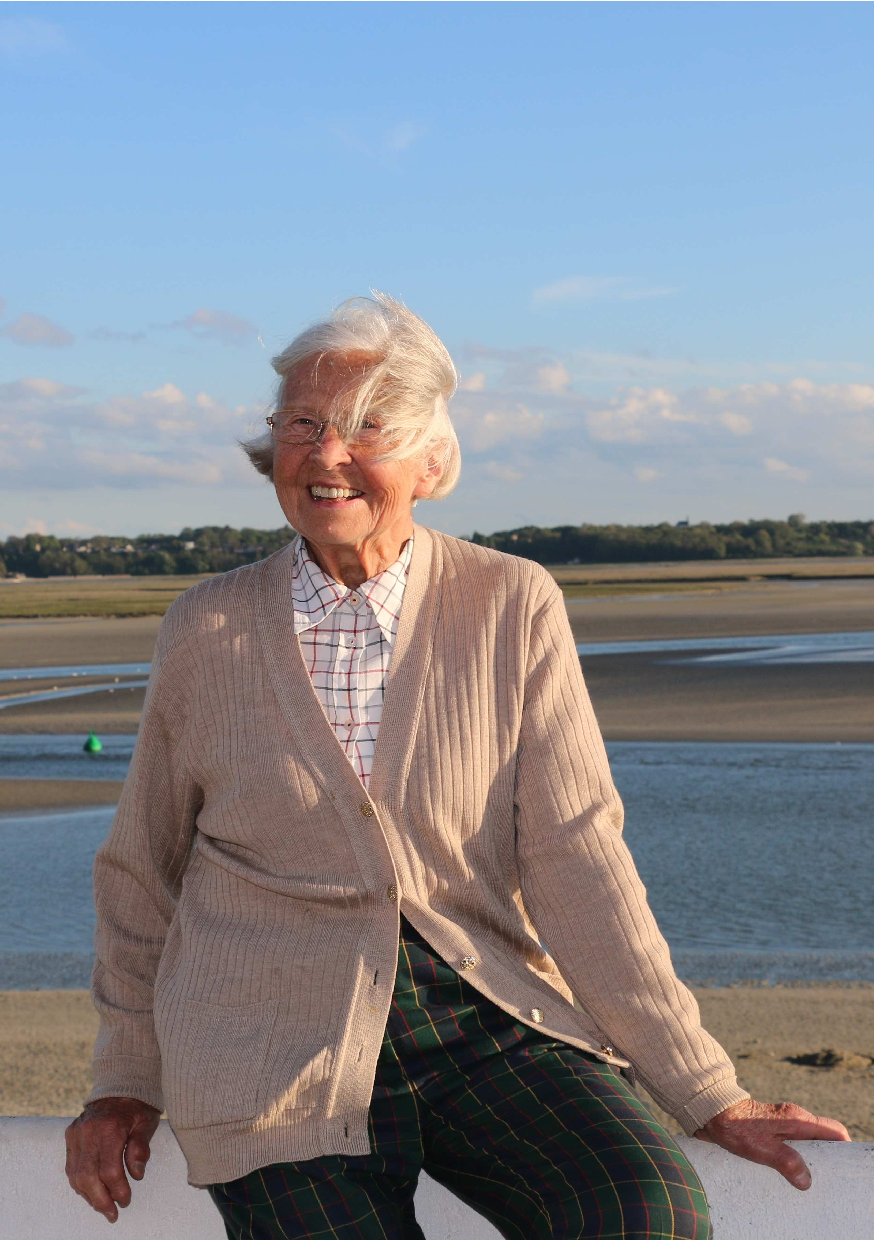
\includepdf{images/4ecouv.pdf}


\end{document}